\documentclass[xcolor={usenames,dvipsnames,svgnames,table}, aspectratio=43]{beamer}
\usepackage[utf8x]{inputenc}
\usepackage[T1]{fontenc}
\usepackage{listings}
\usepackage{listingsutf8}				% package PAS PAR DEFAUT + ? \usepackage{textcomp}

\usepackage{verbatim}
\usepackage{tikz}
\usepackage{tkz-graph}

\usepackage{fancybox}
\setbeamercolor{btcolor}{fg=black,bg=gray}
\usepackage{corse-slides}
\usefonttheme[onlymath]{serif}
\renewcommand{\emph}[1]{{\usebeamercolor[fg]{titlelike}#1}}

%symboles, couleurs, algorithmes
\colorlet{green2}{green!50!black}
\newcommand{\before}{\prec_{\mbox{\scriptsize seq}}}
\newcommand{\violet}[1]{{\color{violet}{#1}}}
\newcommand{\red}[1]{{\color{red}{#1}}}
\newcommand{\blue}[1]{{\color{blue}{#1}}}
\newcommand{\green}[1]{{\color{green2}{#1}}}
\newcommand{\gray}[1]{{\color{gray}{#1}}}
\newcommand{\mysmiley}{\Large \color{red}{\smiley}}
\newcommand{\sad}{\includegraphics[width=1em]{fig/flag-smiley-sad.png}}

\usepackage{fancyvrb}
\usepackage{amsmath,txfonts}
\usepackage{color}
\newcommand{\HI}[1]{\textcolor{gray}{#1}}
\newcommand{\var}[1]{$#1$}
\def\lien{$\multimapdotboth$}

\usepackage{ulem}


%YAML colors
\newcommand\YAMLcolonstyle{\color{red}\mdseries}
\newcommand\YAMLkeystyle{\color{black}\bfseries}
\newcommand\YAMLvaluestyle{\color{blue}\mdseries}

\makeatletter

% here is a macro expanding to the name of the language
% (handy if you decide to change it further down the road)
\newcommand\language@yaml{yaml}

\expandafter\expandafter\expandafter\lstdefinelanguage
\expandafter{\language@yaml}
{
  keywords={true,false,null,y,n},
  keywordstyle=\color{darkgray}\bfseries,
  basicstyle=\YAMLkeystyle\tiny,                                 % assuming a key comes first
  sensitive=false,
  comment=[l]{\#},
  morecomment=[s]{/*}{*/},
  commentstyle=\color{purple}\ttfamily,
  stringstyle=\YAMLvaluestyle\ttfamily,
  moredelim=[l][\color{orange}]{\&},
  moredelim=[l][\color{magenta}]{*},
  moredelim=**[il][\YAMLcolonstyle{:}\YAMLvaluestyle]{:},   % switch to value style at :
  morestring=[b]',
  morestring=[b]",
  literate =    {---}{{\ProcessThreeDashes}}3
                {|}{{\textcolor{red}\textbar}}1 
                {\ -\ }{{\mdseries\ -\ }}3,
}

\usepackage{xspace}

\newcommand{\potrfcolor}[1]{\textcolor{Goldenrod}{\textbf{#1}}\xspace}
\newcommand{\potrf}{\potrfcolor{POTRF}}
\newcommand{\trsmcolor}[1]{\textcolor{blue}{\textbf{#1}}\xspace}
\newcommand{\trsm}{\trsmcolor{TRSM}}
\newcommand{\syrkcolor}[1]{\textcolor{red}{\textbf{#1}}\xspace}
\newcommand{\syrk}{\syrkcolor{SYRK}}
\newcommand{\gemmcolor}[1]{\textcolor{ForestGreen}{\textbf{#1}}\xspace}
\newcommand{\gemm}{\gemmcolor{GEMM}}
% switch to key style at EOL
\lst@AddToHook{EveryLine}{\ifx\lst@language\language@yaml\YAMLkeystyle\fi}
\makeatother

\newcommand\ProcessThreeDashes{\llap{\color{cyan}\mdseries-{-}-}}

\lstset{
	tabsize=4,
%	frame=single,
	breaklines=true,
	basicstyle=\ttfamily\tiny,
	frame=tb,
	framerule=0.2pt,
%	frameround={tttt},
	showstringspaces=false,
	language=c,
%	linewidth=0.95\textwidth,
	keywordstyle=\color{black}\bfseries,
%	keywordstyle=\color{blue},
	commentstyle=\color{OliveGreen},
	stringstyle=\color{red}\itshape,
	inputencoding=utf8/latin1,
	numbers=left,
	numberstyle=\tiny,
	numbersep=5pt,
% OMP define
emph={\#,pragma, taskwait, omp, task, depend, affinity, firstprivate, shared}, emphstyle=\color{RoyalBlue}\bfseries,
emph={[2]in,inout,out,cw,node,thread,data, actions,watchers}, emphstyle={[2]\color{BrickRed}\bfseries},
emph={[3]tied,untied}, emphstyle={[3]\color{Gray}\bfseries},
emph={[4]lu0,fwd,bdiv,bmod}, emphstyle={[4]\color{DarkGreen}\bfseries},
emph={[5]cw}, emphstyle={[5]\color{DarkViolet}\bfseries},
}
\setbeamertemplate{itemize item}[circle]
\setbeamertemplate{section in toc}[circle]
\setbeamertemplate{subsection in toc}[square]
%\setbeamercolor{itemize item}{bg=BrickRed, fg=red}
%\setbeamercolor{section number projected}{bg=BrickRed, fg=white}
%\setbeamercolor{subsection number projected}{bg=BrickRed, fg=white}

\beamertemplatenavigationsymbolsempty
\usepackage{appendixnumberbeamer}

\title[Soutenance de thèse]{Étude et amélioration de l'exploitation des architectures NUMA à travers des supports exécutifs
  \vspace{-25pt}
}
\author[Philippe Virouleau]{
Philippe Virouleau\\
  ~\\
\small Encadrants :\\
François Broquedis, Thierry Gautier, Fabrice Rastello}
\institute[CORSE/AVALON]{Inria - CORSE/AVALON teams}
\date{5 Juin 2018}

%\pgfdeclareimage[height=1cm]{logo-inria-small}{logos/logo-inria}
\titlegraphic{\vspace{-5em}
\includegraphics[height=1cm]{logos/logo-inria}}

\begin{document}

% intro blabla
% intro cholesky
% intro observation perfs, gant, distrib
% point méthodo, intro plan
% 15 min là
% carton + 8
% runtime + 12
% simu+conclusion + 10
%TODO : à chaque fin de parties : point positionnement

%TODO: T=#inst * cycle/#inst * 1/freq
%algo, vector,numa, hardware
%TODO: carton, dgemm avec distribution random sur au moins 16 et 192 (pour : plot distribution et regarder les pics, et comparer au min perf du simu)


% Je pense partir sur un plan similaire à ma thèse :
% - task dep (cholesky)
% - Architecture cible et modèle de programmation
%   - NUMA
% - Caractérisation
%   - Description de l'outil et motivation
%   - chiffre cholesky
%   - enchainement motivation extension
% - Extensions
%   - OpenMP
%   - support exécutif
%   - Perf
% - Travaux en cours
%   - blabla simu + julien


\AtBeginSection[]
{
  \begin{frame}
     \frametitle{Plan}
     \tableofcontents[currentsection]
  \end{frame}
}
%\AtBeginSubsection[]
%{
      %\begin{frame}
          %\frametitle{Outline}
              %\tableofcontents[currentsection,currentsubsection]
                %\end{frame}
%}



\mymaketitle
%\maketitle

\begin{frame}
\frametitle{Contexte}
blabla appli simulation jolie image
\end{frame}

\begin{frame}
\frametitle{Contexte}
blabla schéma supercalculateur, zoom sur un noeud du cluster
\end{frame}

\begin{frame}
\frametitle{Contexte}
blabla péage (caisse, voitures plus ou moins lente à passer, donc faudrait pouvoir les bouger)
=> analogie en remplaçant les caisses par des coeurs, les voitures par des taches

=> transition application à base de tâche
\end{frame}

\begin{frame}
\frametitle{Une application omniprésente : Cholesky}

Factorisation d'une matrice symétrique positive définie $A$ : 
$$ A = L*L^T$$

\begin{itemize}
\item Très utilisée pour la résolution de systèmes d'équations.

\item Plusieurs versions : choix d'une version parallèle par bloc.
\end{itemize}

\end{frame}

\begin{frame}[fragile]
\frametitle{Une application omniprésente : Cholesky}

Description des opérations et de leur ordre :

\noindent{%
\begin{minipage}[t]{0.38\linewidth}
  \begin{block}{Noyaux:}
    \begin{itemize}
      \item \potrf Cholesky
      \item \trsm Résolution d'un système triangulaire
      \item \gemm Multiplication de matrices
      \item \syrk Multiplication de matrices symétriques
    \end{itemize}
  \end{block}
\end{minipage}}%
\hfill%
\begin{minipage}[t]{0.54\linewidth}
  \begin{figure}
    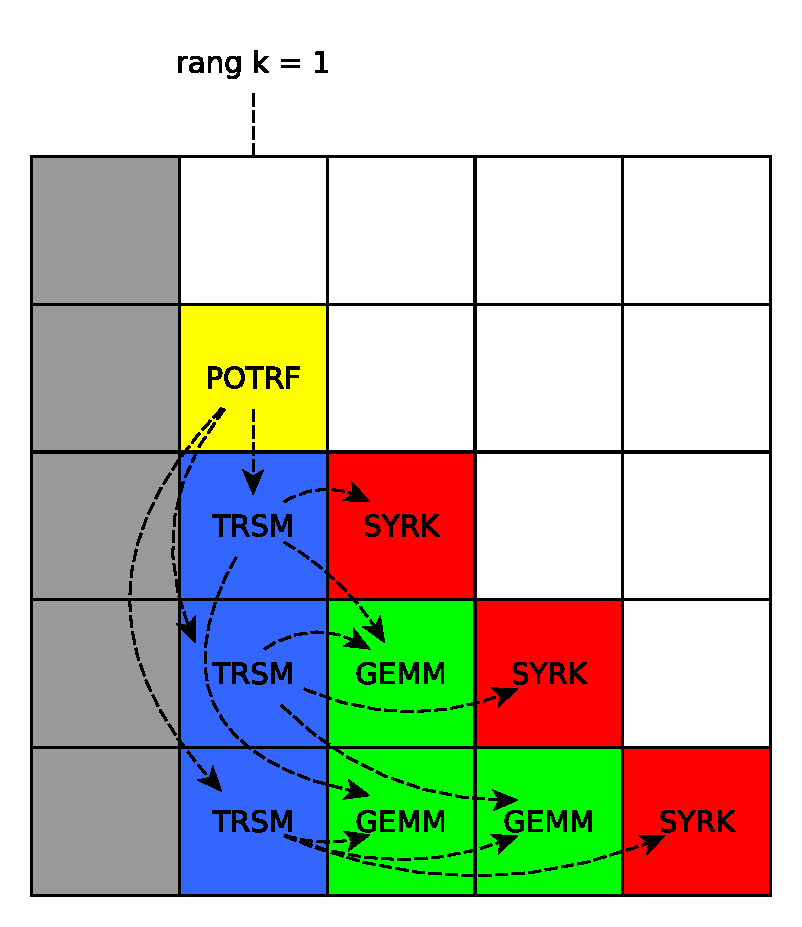
\includegraphics[width=\textwidth]{graph/cholesky-rank-update.pdf}
  \end{figure}
\end{minipage}


\end{frame}

\begin{frame}
\frametitle{Une application omniprésente : Cholesky}

Exprimée dans un langage par flot de données, et représentation de l'application sous forme de graphe :
\begin{figure}
  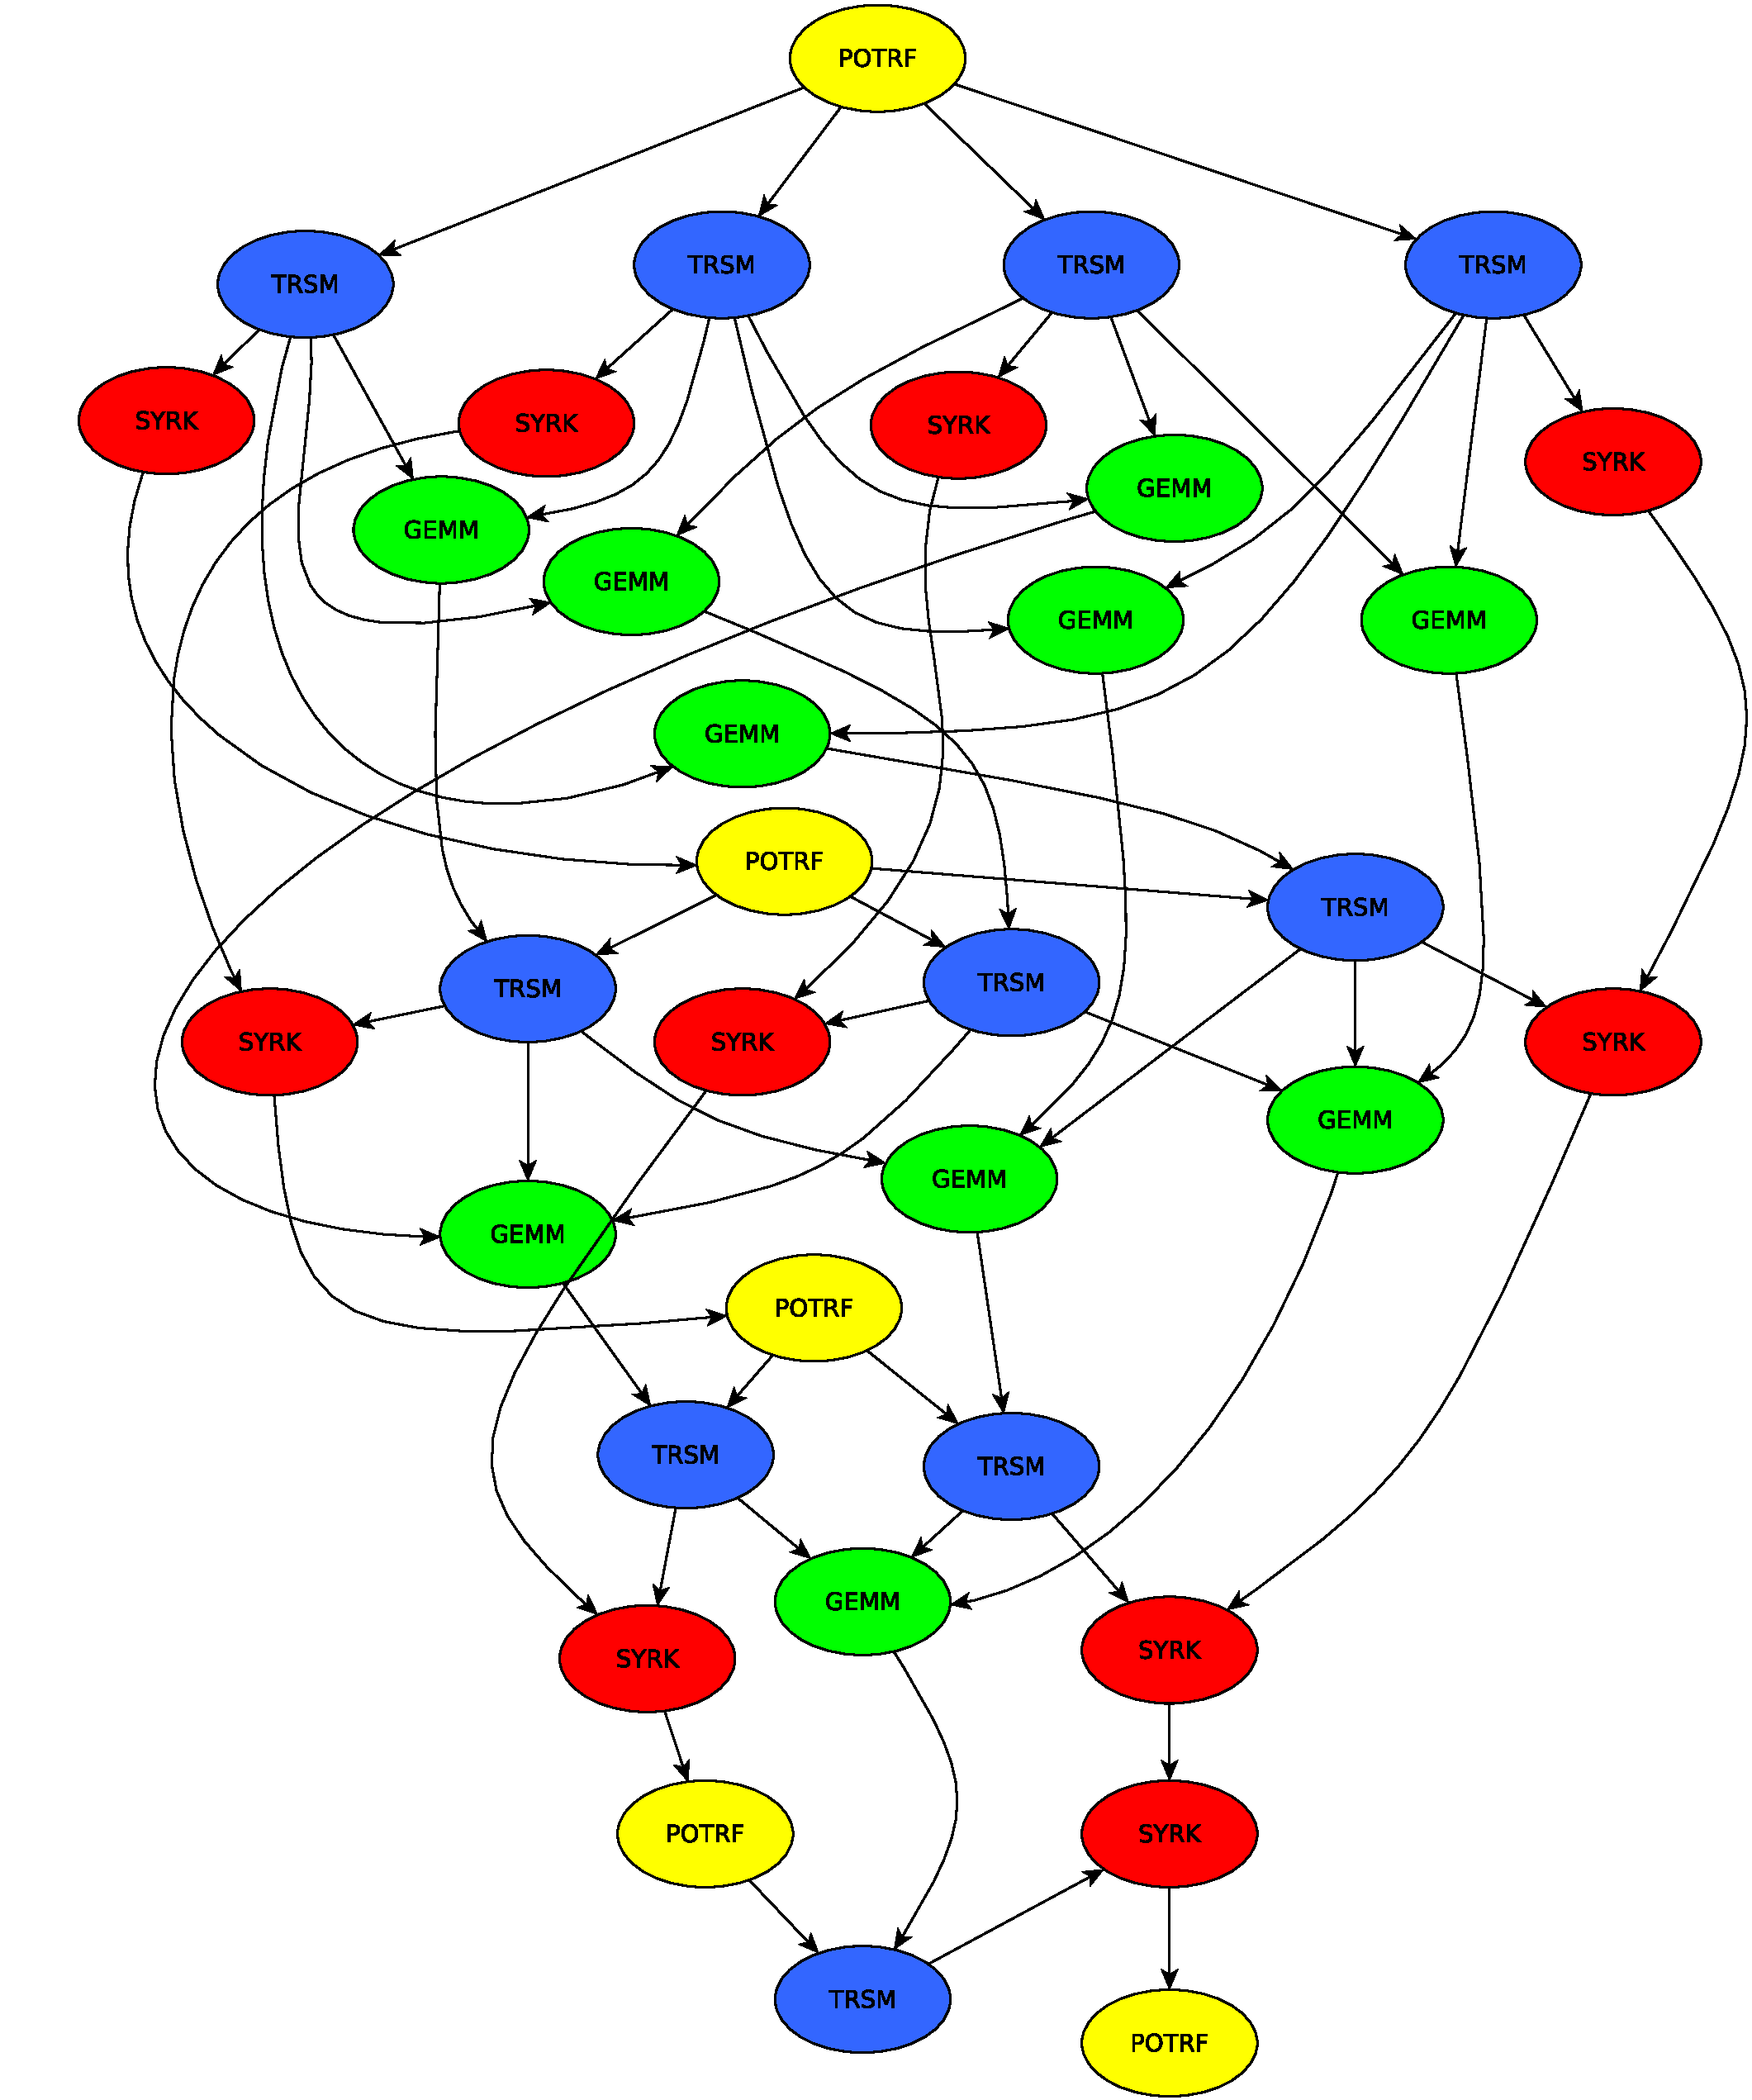
\includegraphics[width=0.4\textwidth]{graph/cholesky-dag-5.pdf}
\end{figure}
TODO : faire une présentation des tâches avec dépendances d'openmp ?


\end{frame}

\begin{frame}
\frametitle{Cholesky : premières observations}

Conditions d'expérience :
\begin{itemize}
  \item Version OpenMP par bloc de Cholesky (KASTORS, tâches avec dépendances)
  \item Support exécutif libKOMP
  \item Machine à mémoire partagée de 192 coeurs
\end{itemize}

Observations :
\begin{itemize}
  \item Performances brutes
  \item Déroulement de l'application
  \item Statistiques sur les différents types de tâches
\end{itemize}

Choix arbitraire d'un cas particulier : matrice de largeur 8192, avec une bonne taille de bloc pour ce cas : 224.

\end{frame}

\begin{frame}
  \frametitle{Cholesky : performances brutes (8192, 224)}

  Évolution de la performance (Gflops) en fonction du nombre de coeurs.

\begin{figure}
  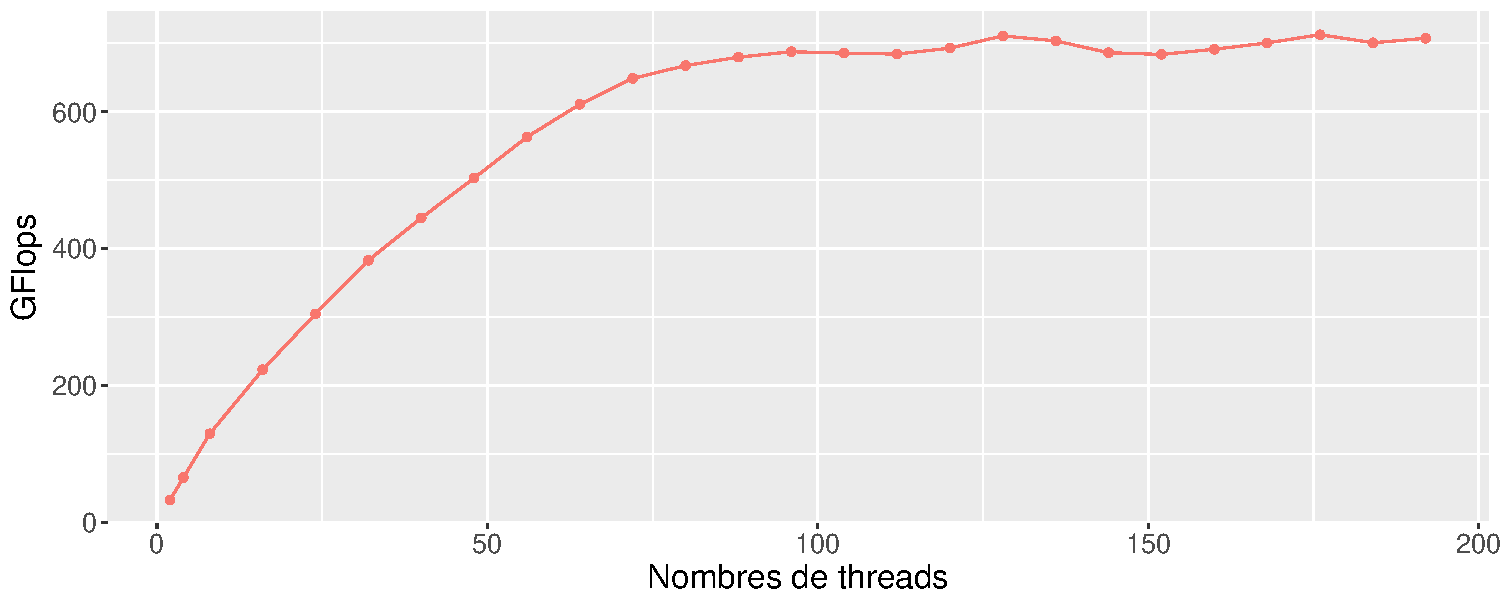
\includegraphics[width=\textwidth]{graph/graph_evolution_cholesky_8192_224.pdf}
\end{figure}
\uncover<2> {
  \begin{block}{Conclusions}
    Peu de conclusion à tirer : bon speedup jusqu'à ~70 coeurs, puis plateau potentiellement du au parallélisme limité.
  \end{block}
}

\end{frame}

\begin{frame}
\frametitle{Cholesky : déroulement de l'application}

Aperçu d'un diagramme de Gantt sur 64 threads
\begin{figure}
  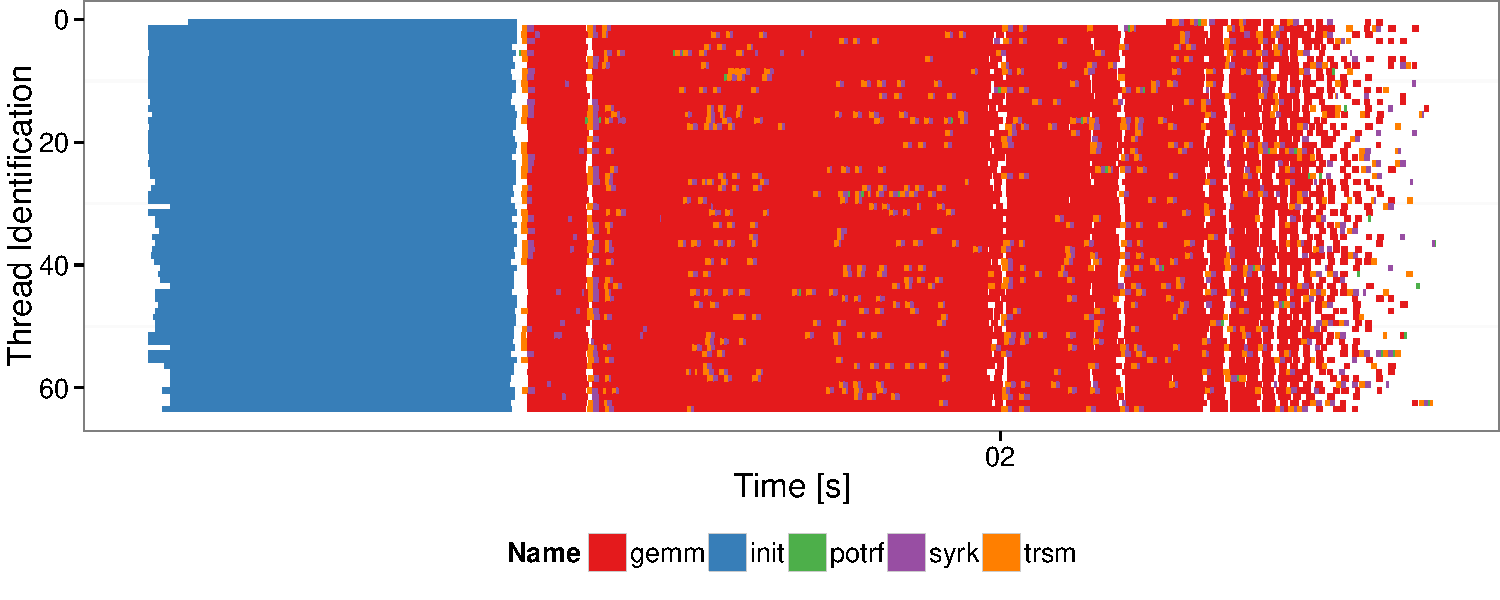
\includegraphics[width=\textwidth]{graph/gantt_8192_224.pdf}
\end{figure}
\uncover<2> {
  \begin{block}{Conclusions}
    Bonne utilisation des ressources, "trous" dûs à l'absence de tâches à différents moments de la vie de l'application.
  \end{block}
}

\end{frame}

\begin{frame}
\frametitle{Cholesky : comportement des différents types de tâches}
\begin{figure}
  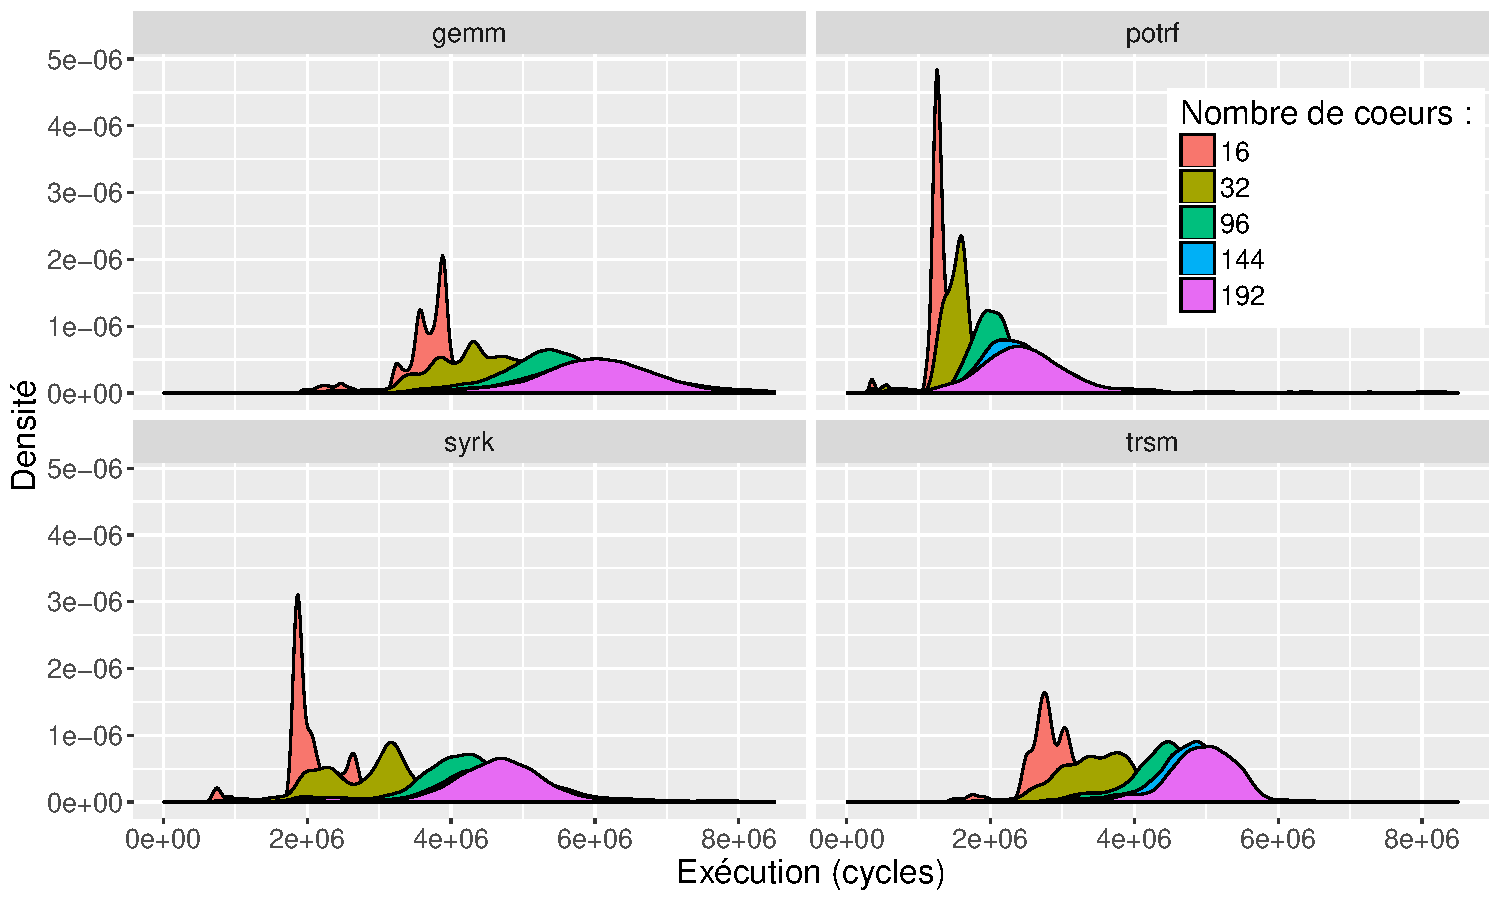
\includegraphics[width=0.8\textwidth]{graph/graph_distrib_overview_8192_224.pdf}
\end{figure}
\uncover<2> {
  \begin{block}{Conclusions}
    Nombre de threads qui augmente $=>$ augmentation du temps moyen d'une tâche et de la variabilité.
  \end{block}
}
\end{frame}


%TODO: T=#inst * cycle/#inst * 1/freq
%algo, vector,numa, hardware
\begin{frame}
  \frametitle{Source(s) des différences de performances}

  \begin{block}{Décomposition d'une tâche}
    $$ T_{total} = \overbrace{N_{instructions}}^\text{\uncover<2->{Algorithme}} * \underbrace{\frac{cycle}{N_{instructions}}}_\text{\uncover<4>{Vectorisation, localité des données}} * \overbrace{\frac{Secondes}{cycle}}^\text{\uncover<3->{Fréquence}} $$
  \end{block}

  \begin{block}{Leviers possibles}
    \begin{itemize}
      \uncover<2->{
	\item Algorithme : fixe, non modifiable.
      }
      \uncover<3->{
	\item Fréquence : fixe, non modifiable.
      }
      \uncover<4>{
	\item Vectorisation : dépendante du compilateur, non modifiable.
	\item Localité des données : clé du problème.
      }
    \end{itemize}
  \end{block}

\end{frame}

\begin{frame}
\frametitle{Localité des données : aperçu d'une machine NUMA}
%Texte : dire ce que ça veut dire NUMA, que les données sont partagées, décrire idchire
\begin{columns}[T,onlytextwidth]
  \column{0.42\textwidth}
  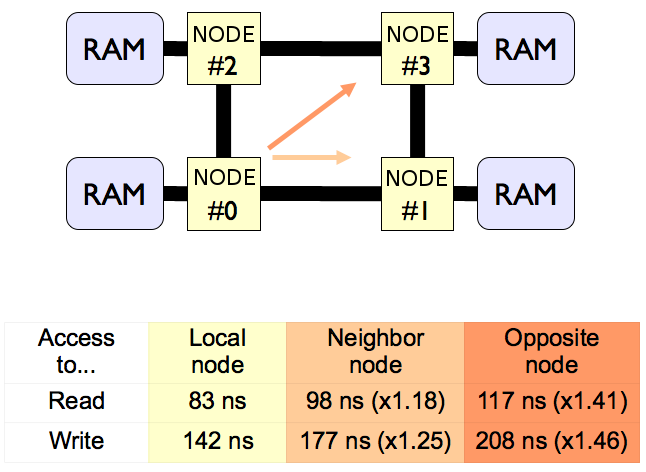
\includegraphics[scale=0.3]{graph/NUMA-latences}
  \column{0.40\textwidth}

  \begin{block}{Description}
    \begin{itemize}
      \item Mémoire partagée
      \item Machine = plusieurs noeuds
      \item Noeud = plusieurs coeurs + une sous partie de la RAM
    \end{itemize}
  \end{block}

\end{columns}
\begin{alertblock}{Conséquence principale}
  Le temps d'exécution d'une tâche dépend de son placement et du placement de ses données
\end{alertblock}

\end{frame}


\begin{frame}
  \frametitle{Méthodologie pour l'amélioration d'une application}
  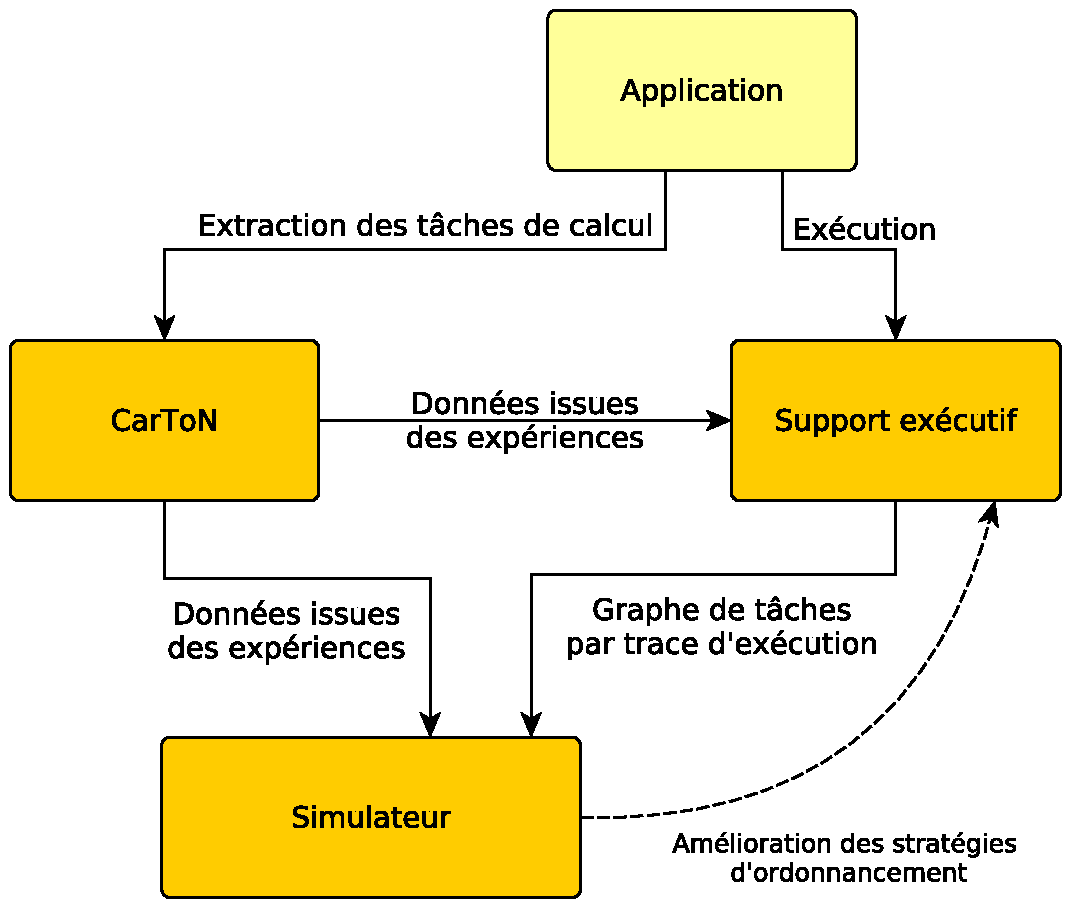
\includegraphics[width=0.8\textwidth]{graph/big_picture.pdf}
\end{frame}

\begin{frame}
  \frametitle{Plan}
  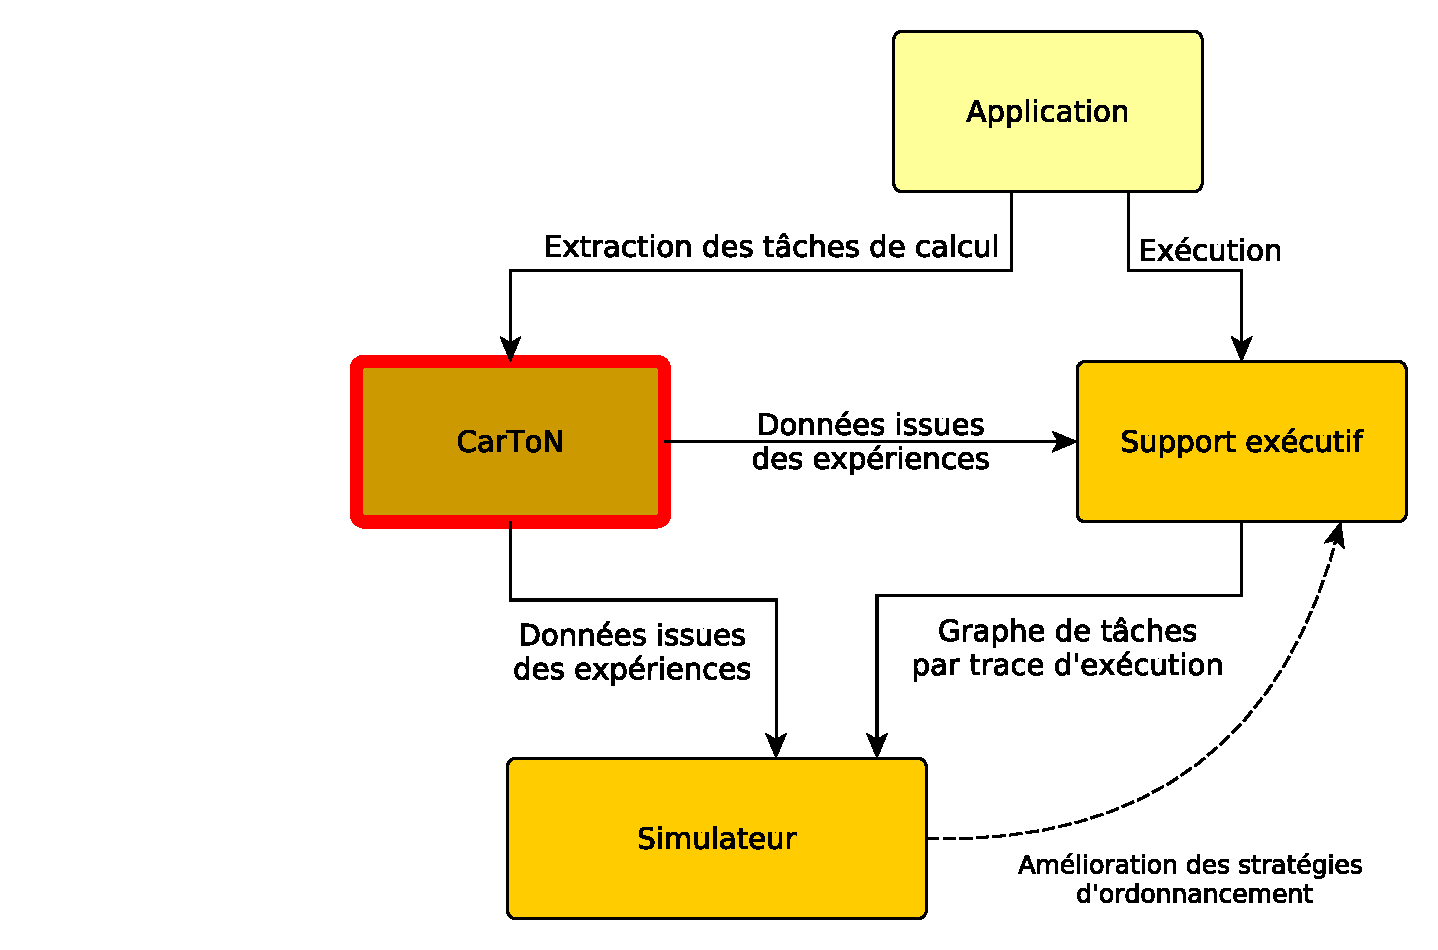
\includegraphics[width=0.8\textwidth]{graph/big_picture-part1.pdf}
\end{frame}


\begin{frame}
\frametitle{Travaux existants}

Objectif : pouvoir exécuter des portions de code arbitraire, avec une connaissance et un contrôle sur le placement des données manipulées.

\begin{itemize}
  \item Benchmarks, microbenchmarks
    
    \emph{beaucoup} de travaux existants, mais aucun adapté

  \item Autres outils

    BOAST : autotuning de noyaux applicatifs.
\end{itemize}

\end{frame}

\begin{frame}
  \frametitle{CarToN : Characterization Tool for NUMA architectures}

  \begin{block}{Objectifs et motivations}
    \begin{itemize}
      \item Observer et comprendre le comportement d'un noyau applicatif arbitraire
      \item Pas (peu) d'interférence liée à l'exécution
    \end{itemize}
  \end{block}

  \begin{block}{Éléments de base}
    Un "scénario" décrivant :
    \begin{itemize}
      \item Données (ex: matrice A, B)
      \item Actions (ex: B=A+B)
      \item Paramètres à observer (ex: flops, cache miss, ...)
    \end{itemize}
  \end{block}

  \begin{block}{Modèle d'exécution}
    Une queue FIFO par coeurs, création et enfilement des tâches à la lecture du scénario.
  \end{block}
\end{frame}

\begin{frame}[fragile]
\frametitle{Exemple de scénario : exécution de 8 GEMM indépendant}

\hspace{0.1cm}
\begin{minipage}[t]{0.38\linewidth}
  Déclaration des données
  \begin{lstlisting}[language=yaml]
data:
  size:
    type: int
    value: 256
  a<i>:
    i: [0, 7, 1]
    type: double*
  b<i>:
    i: [0, 7, 1]
    type: double*
  c<i>:
    i: [0, 7, 1]
    type: double*
  \end{lstlisting}
\begin{uncoverenv}<3->
  Paramètres à observer
  \begin{lstlisting}[language=yaml]
watchers:
- name: flops_dgemm
  params:
  - size
  kernels:
  - dgemm
  \end{lstlisting}
\end{uncoverenv}
\end{minipage}
\hspace{0.3cm}
\begin{uncoverenv}<2->
\begin{minipage}[t]{0.54\linewidth}
  Déclaration des actions
  \begin{lstlisting}[language=yaml]
actions:
- for:
  var: i
  limits: [0, 7, 1]
  actions:
  - for:
    var: name
    values: ["a", "b", "c"]
    actions:
    - kernel: init_blas_bloc
      core: <i>
      params: "<name><i>", "size"
- kernel: barrier
- for:
  var: i
  limits: [0, 7, 1]
  actions:
  - kernel: dgemm
    core: <i>
    repeat: '50'
    params: ["a<i>", "b<i>", "c<i>", "size"]
  \end{lstlisting}
\end{minipage}
\end{uncoverenv}

\end{frame}

\begin{frame}
\frametitle{Applications aux noyaux de Cholesky}

\begin{block}{Objectif}
  Analyser le comportement des quatres noyaux de l'application (\potrf, \trsm, \syrk, \gemm).

  Conditions d'expérience :
  \begin{itemize}
    \item exécutions sur des données \emph{indépendantes}
    \item placement des données (locales, distantes)
    \item charge de la machine (nombre d'exécutions concurrentes)
  \end{itemize}
\end{block}

\end{frame}

\begin{frame}
\frametitle{Applications aux noyaux de Cholesky}

Présenter les deux cas de base (faire varier la localité et la charge de la machine)

\end{frame}

\begin{frame}
\frametitle{Applications aux noyaux de Cholesky}

Présenter les deux cas de base (faire varier la localité et la charge de la machine)

\end{frame}

\begin{frame}
\frametitle{Applications aux noyaux de Cholesky}

eval de perf 1 (comparaison noyaux, impact de la charge)

\end{frame}

\begin{frame}
\frametitle{Applications aux noyaux de Cholesky}

eval de perf 2 (local vs distant, +impact sortie du cache)

\end{frame}

\begin{frame}
\frametitle{Applications aux noyaux de Cholesky}

eval de perf 3 : distrib des temps noyaux avec init "random" => TODO !

\end{frame}

\begin{frame}
  \frametitle{Conclusion}
  \begin{block}{Remarques}
    Triple effet sur les performances :
    \begin{itemize}
      \item Baisse linéaire des perfs. (débit limité, concurrence sur les caches ?)
      \item Différence local vs distant.
      \item Différence d'impact de la localité 256 vs 512 (données ne tiennent pas dans le L3 pour 512).
    \end{itemize}
  \end{block}

  \begin{block}{Motivation}
    Régler le plus gros problème : la localité.
  \end{block}

\end{frame}

\begin{frame}
\frametitle{Synthèse}

on a de quoi tout bien définir, on peut :
- partir sur la localité dans le runtime direct
- nourrir un simulateur

\end{frame}

\begin{frame}
  \frametitle{Plan}
  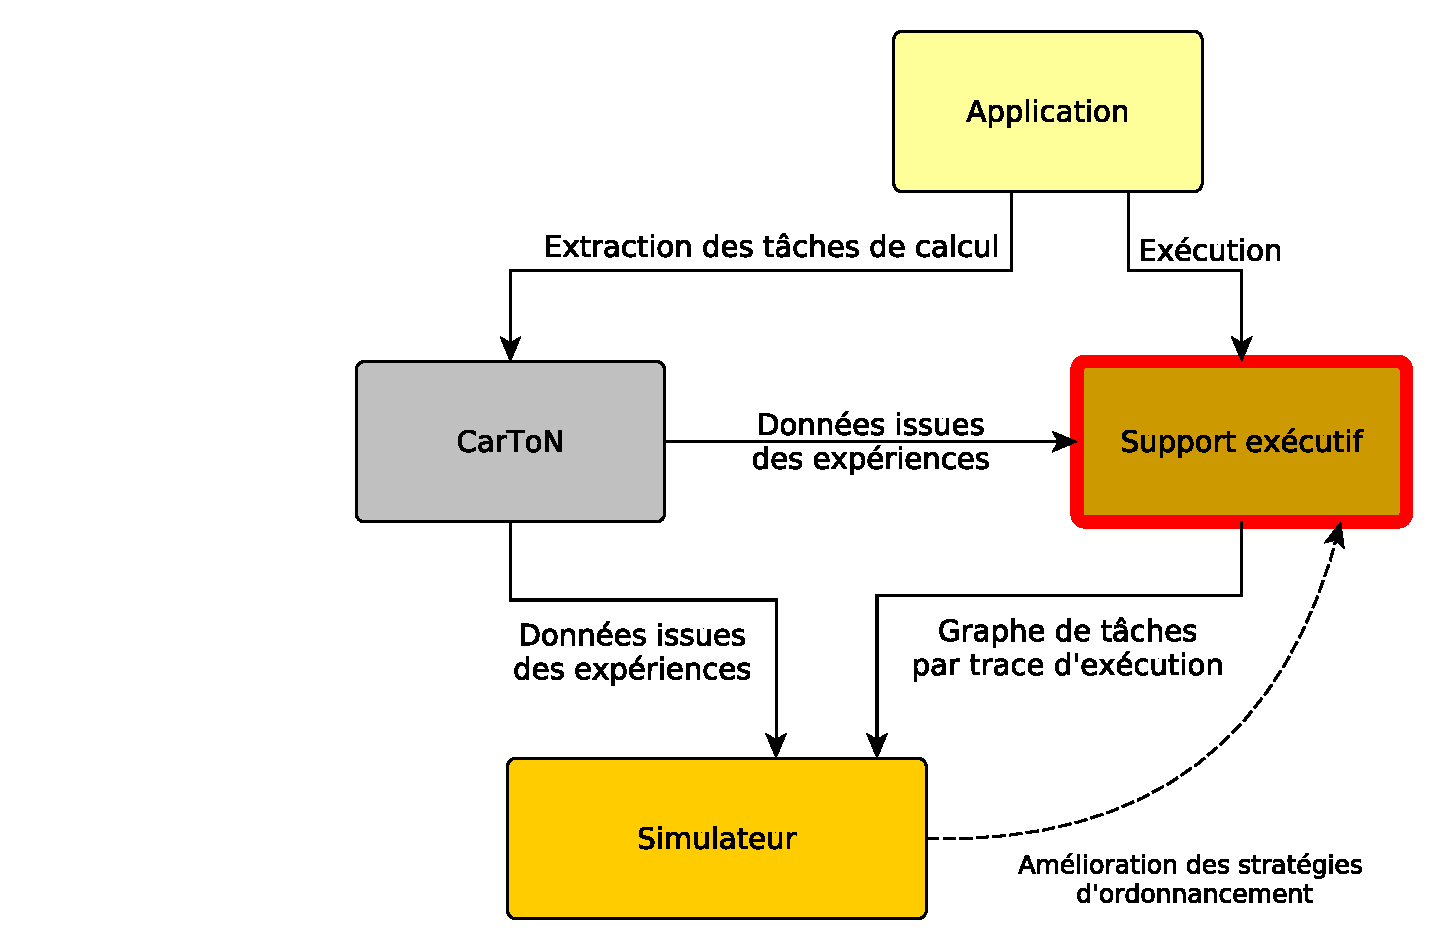
\includegraphics[width=0.8\textwidth]{graph/big_picture-part2.pdf}
\end{frame}


\begin{frame}
\frametitle{Fonctionnement}

Rappel : application représentée sous forme de DAG

\begin{figure}
  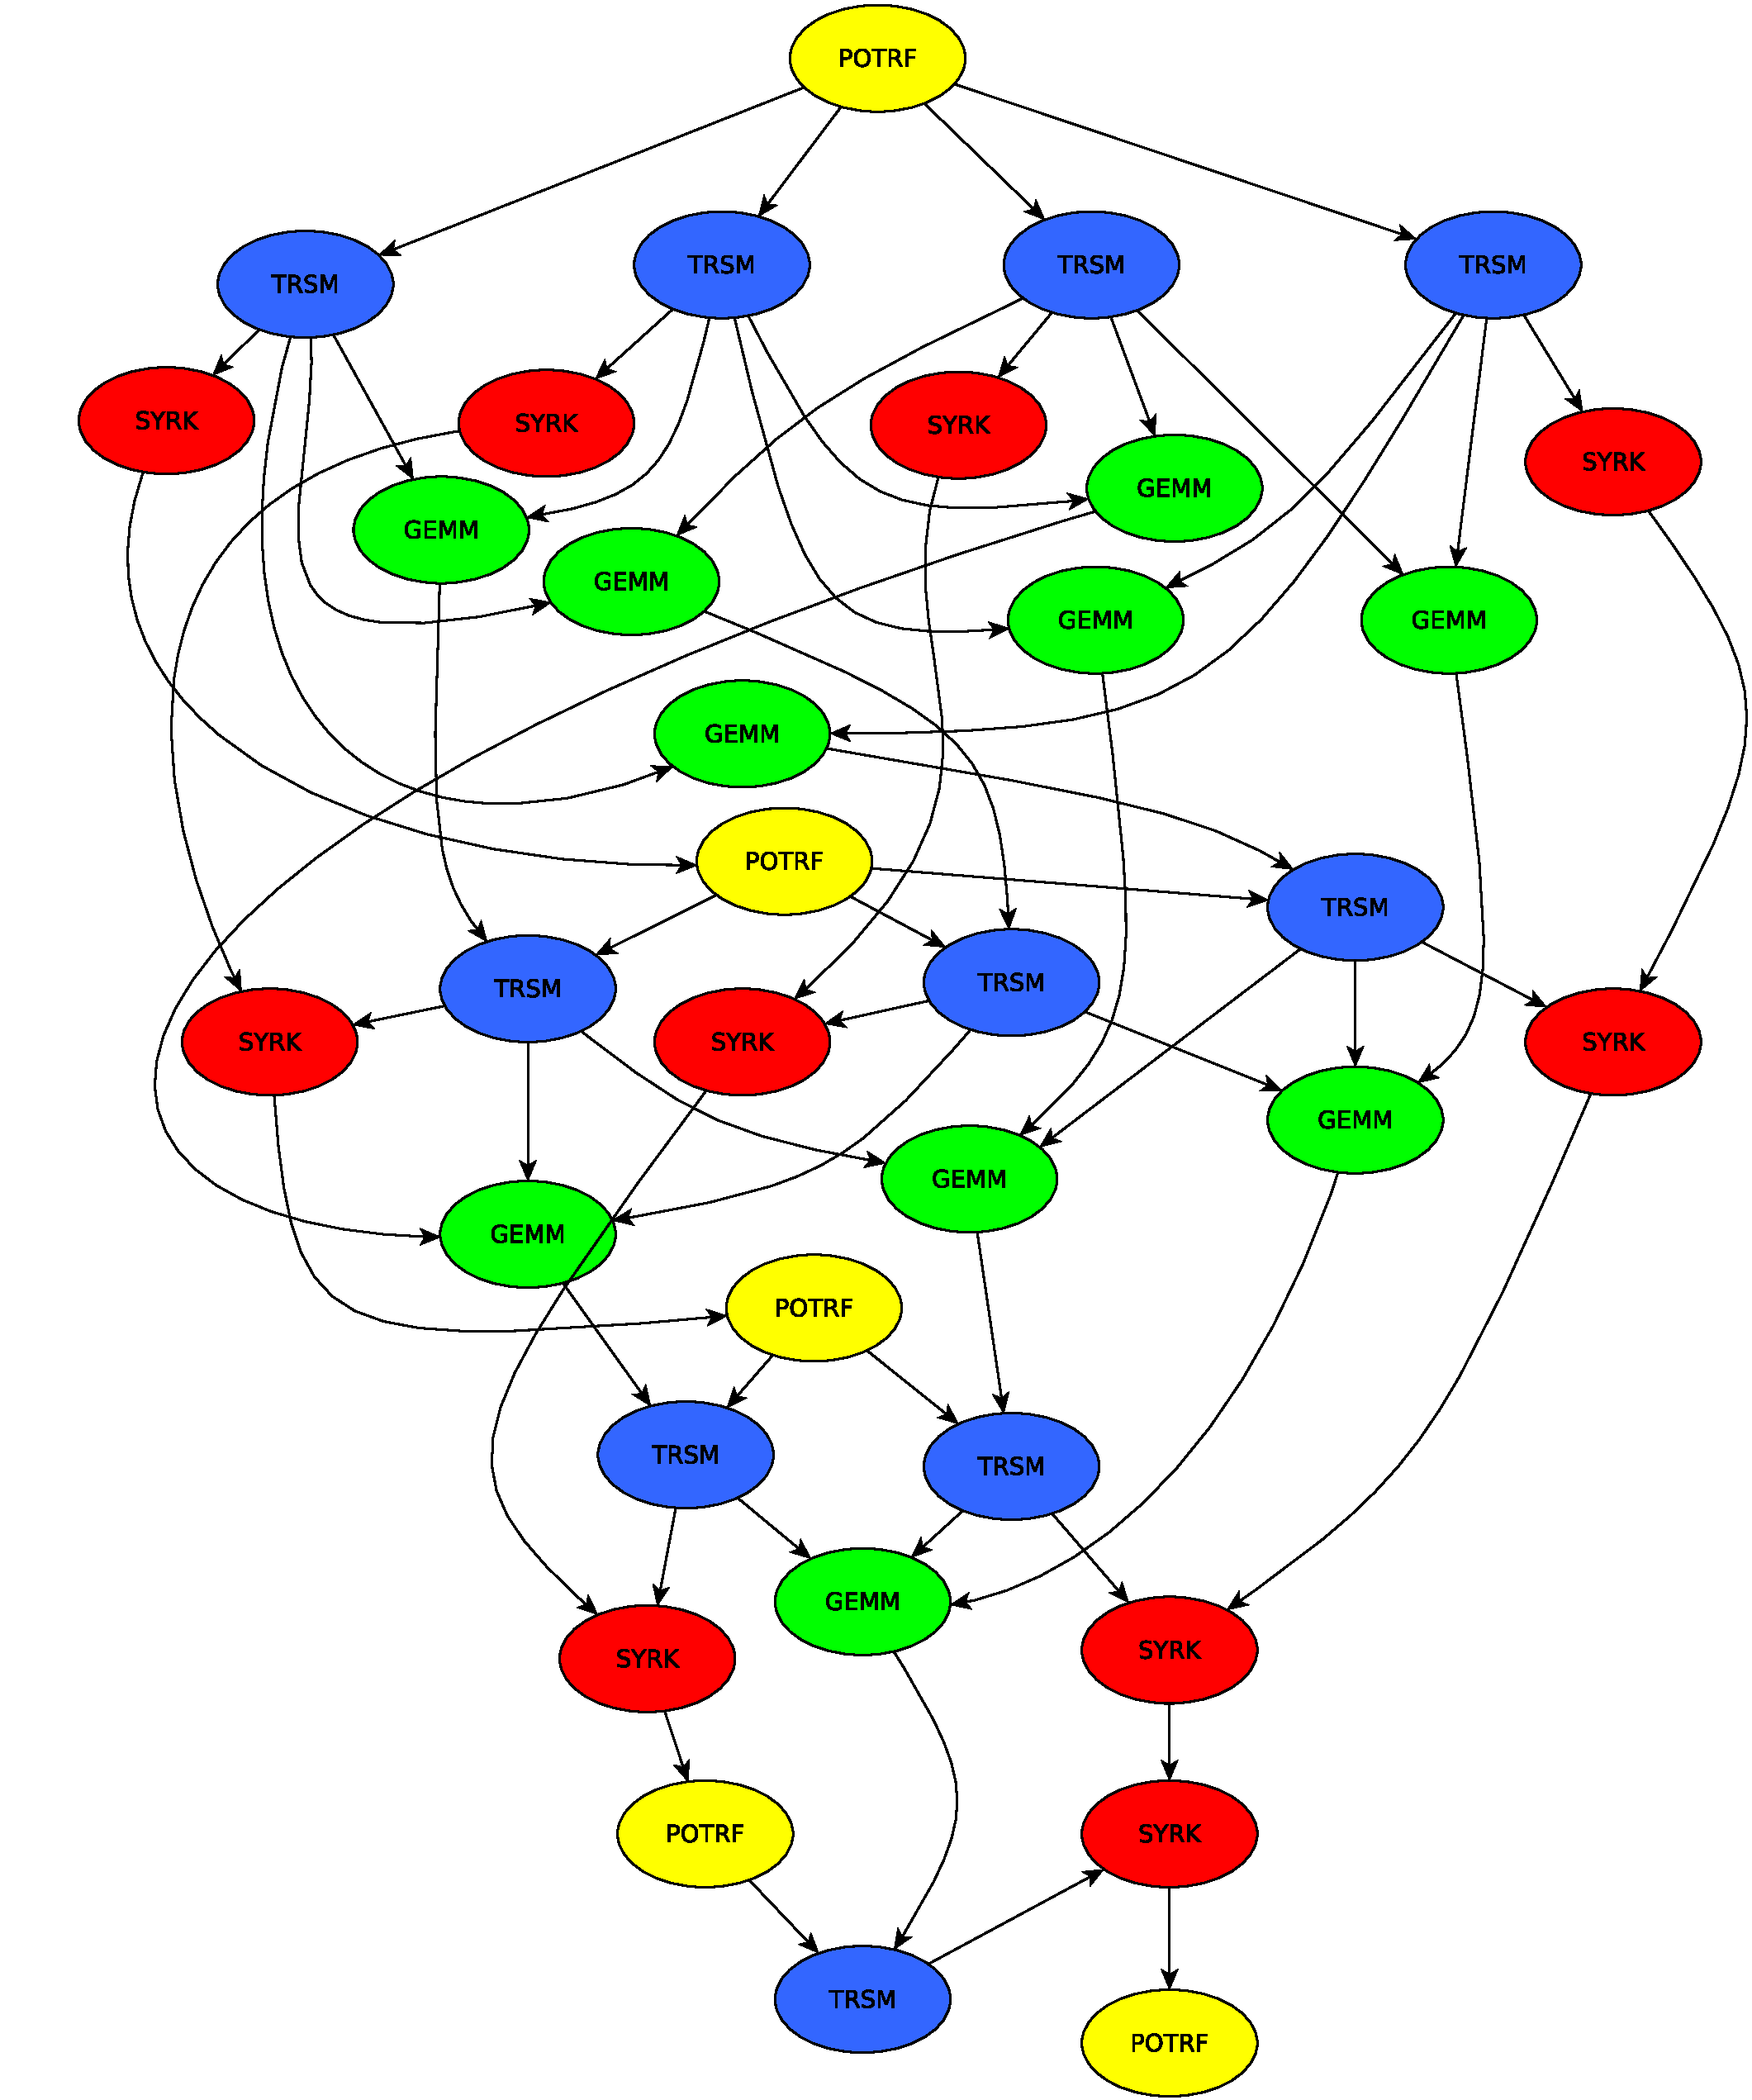
\includegraphics[width=0.4\textwidth]{graph/cholesky-dag-5.pdf}
\end{figure}

\end{frame}



\begin{frame}[fragile]
\frametitle{Approches pour l'amélioration de la localité}

  \begin{block}{En amont}
    \begin{itemize}
      \item Extension OpenMP pour le programmeur :

        \verb/affinity/ entre une tâche et ses données.
    \end{itemize}
  \end{block}

  \begin{block}{Pour le support exécutif}
    \begin{itemize}
      \item Vision hiérarchique de la machine
      \item Ordonnancement prenant en compte la localité des données (données fournies par le programmeur, informations dans les dépendances)
    \end{itemize}
    Modèle d'exécution : vol de travail.
  \end{block}

\end{frame}

\begin{frame}[fragile]
\frametitle{Influencer la localité des données : l'affinité}

Donner le moyen au programmeur de passer des informations au support exécutif.

\begin{block}{Introduction d'une clause OpenMP pour l'affinité}
  Clause attachée à une tâche :
  \begin{lstlisting}[numbers=none, basicstyle=\normalsize]
  affinity([node | thread | data]: expr[, strict])
  \end{lstlisting}
\end{block}
\begin{block}{À quoi \texttt{expr} fait référence}
  \begin{itemize}
    \item \texttt{thread} -> indice d'un thread
    \item \texttt{node} -> indice d'un noeud NUMA
    \item \texttt{data} -> adresse mémoire
  \end{itemize}
\end{block}


\end{frame}

\begin{frame}
\frametitle{Support exécutif : maintient des tâches prêtes}

  Le support exécutif possède une file de tâches prêtes par élément de la hiérarchie.

\begin{figure}
  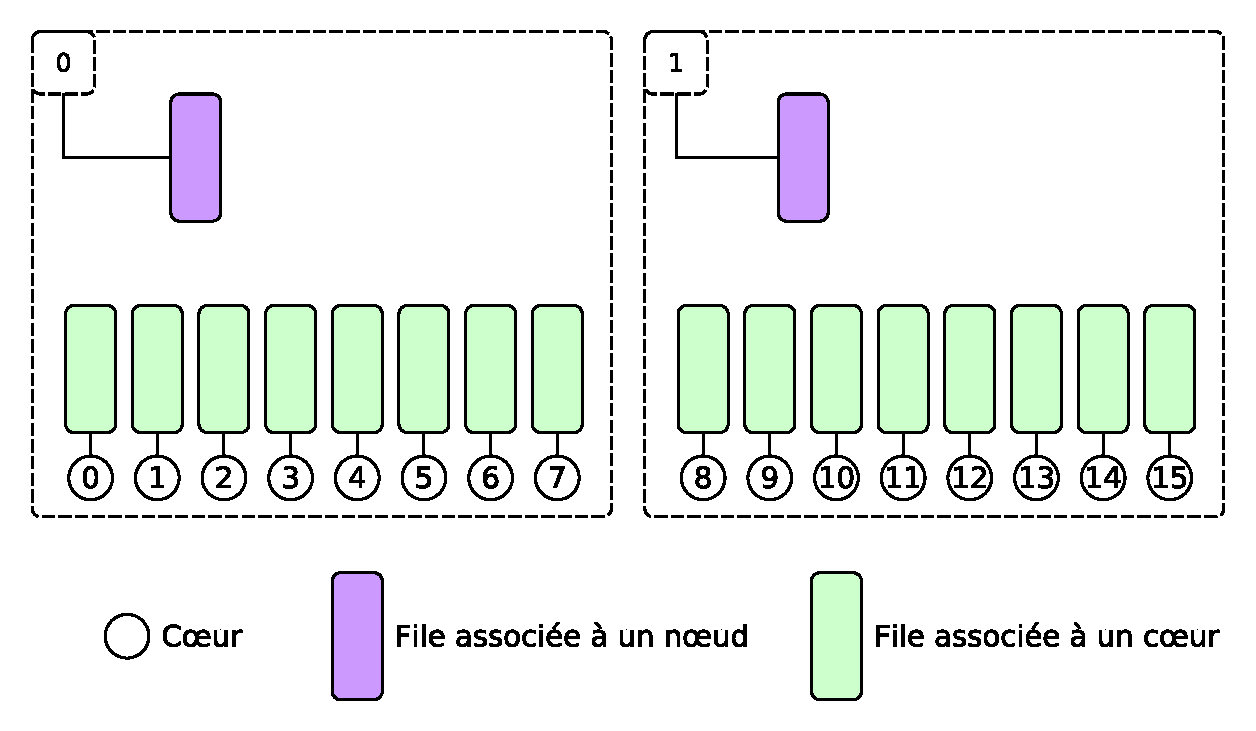
\includegraphics[width=0.8\textwidth]{graph/hierarchical_queues.pdf}
\end{figure}
\end{frame}

\begin{frame}[fragile]
\frametitle{Support exécutif : le vol de travail}

\begin{columns}[T,onlytextwidth]
  \column{0.60\textwidth}
  \vspace{1cm}

  \textbf{Vol de travail : deux étapes majeures}
  \begin{itemize}
    \item Workers \textit{poussent} une tâche dans une queue
    \item Voleurs \textit{sélectionnent} une queue où voler
  \end{itemize}
  \column{0.4\textwidth}
  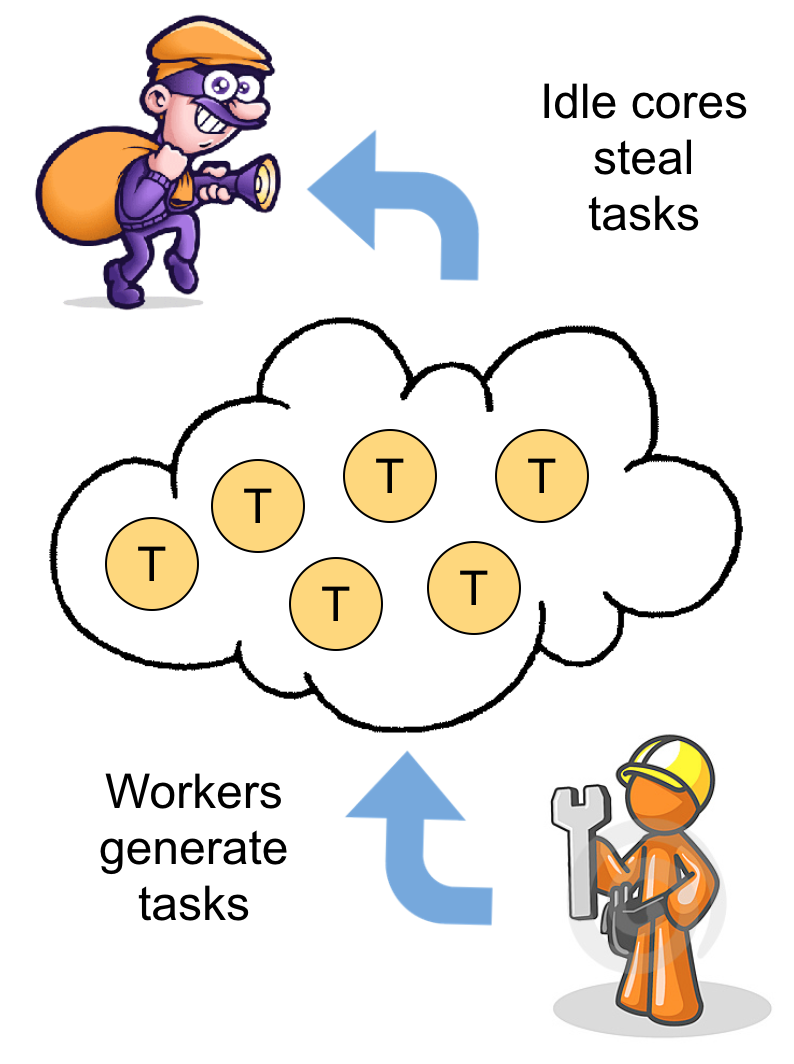
\includegraphics[scale=0.38]{graph/ws}
\end{columns}

\end{frame}

\begin{frame}
\frametitle{Exemple de stratégies d'ordonnancement}

\vspace{0.3cm}
Sélection d'une queue pour le placement d'une tâche prête
\begin{itemize}
  \item Si affinité : placement sur le noeud possédant la donnée, ou dans la queue du coeur si celui si est sur le noeud
  \item Sinon placement dans la queue du coeur locale
\end{itemize}
\vspace{0.5cm}

Sélection d'une queue pour le vol
\begin{figure}
  \only<2> {%
    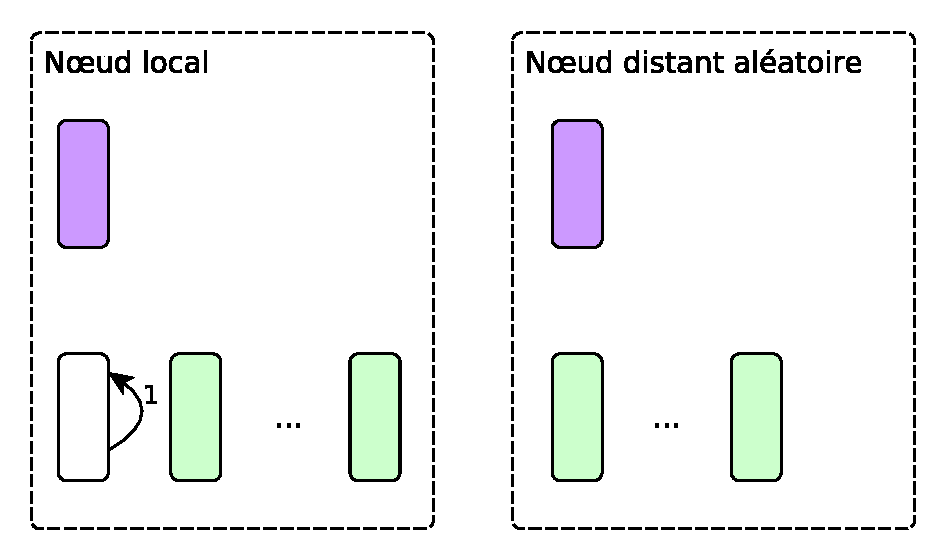
\includegraphics[width=0.6\textwidth]{graph/steal_strategies_anim_1.pdf}%
  }%
  \only<3> {%
    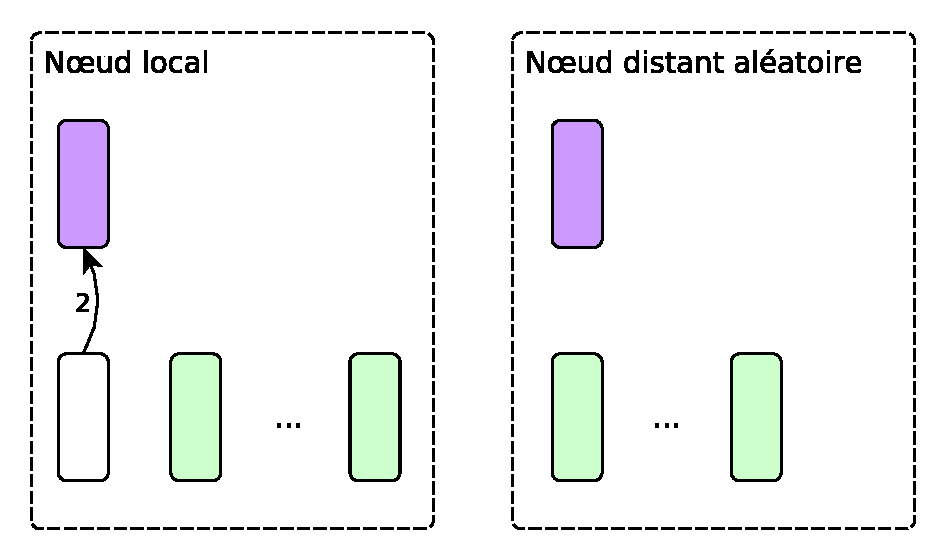
\includegraphics[width=0.6\textwidth]{graph/steal_strategies_anim_2.pdf}%
  }%
  \only<4> {%
    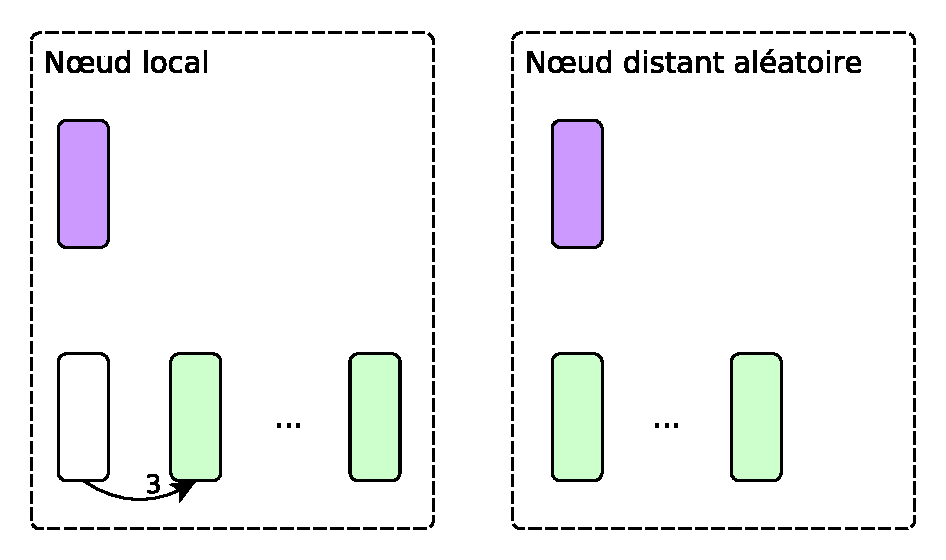
\includegraphics[width=0.6\textwidth]{graph/steal_strategies_anim_3.pdf}%
  }%
  \only<5> {%
    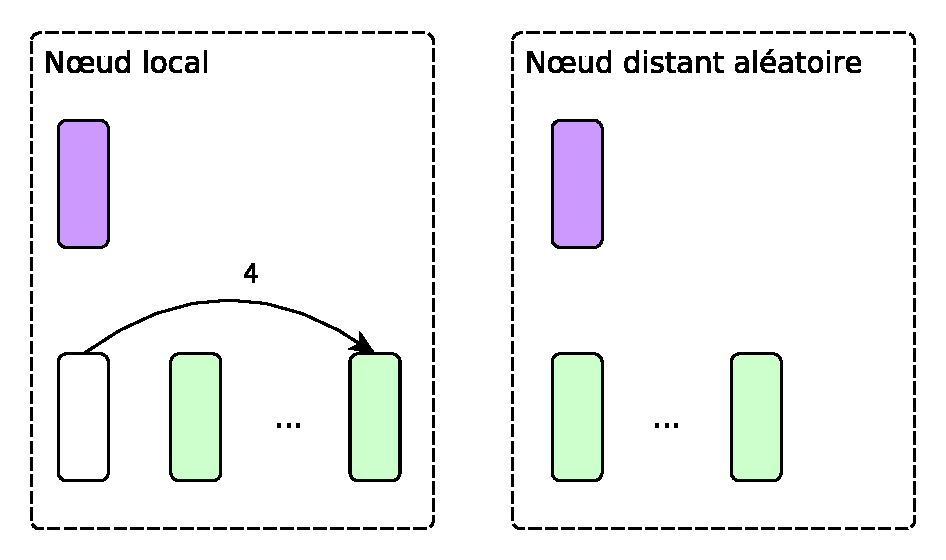
\includegraphics[width=0.6\textwidth]{graph/steal_strategies_anim_4.pdf}%
  }%
  \only<6> {%
    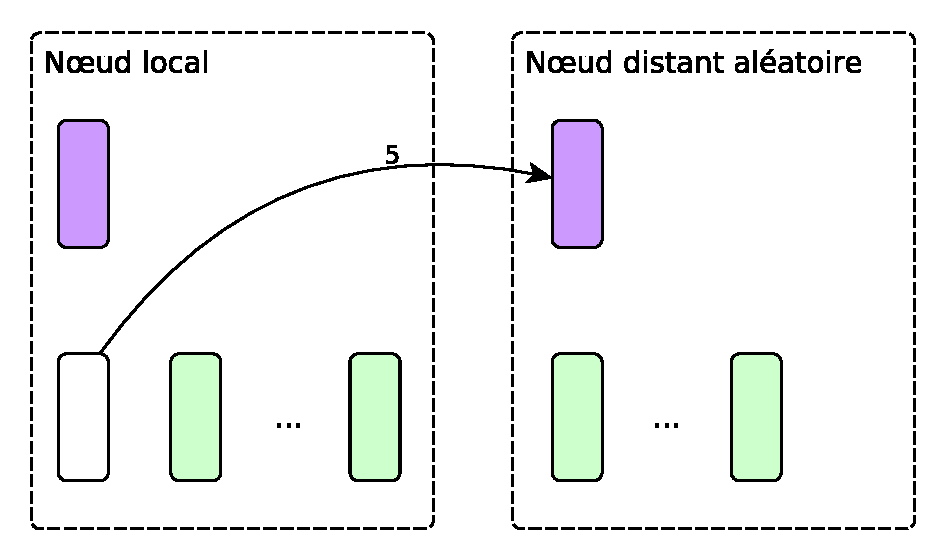
\includegraphics[width=0.6\textwidth]{graph/steal_strategies_anim_5.pdf}%
  }%
  \only<7> {%
    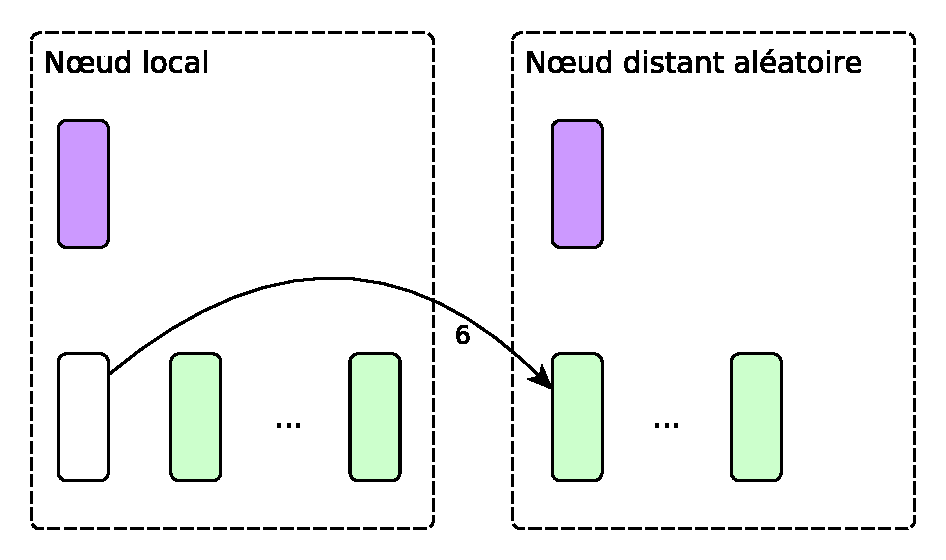
\includegraphics[width=0.6\textwidth]{graph/steal_strategies_anim_6.pdf}%
  }%
  \only<8> {%
    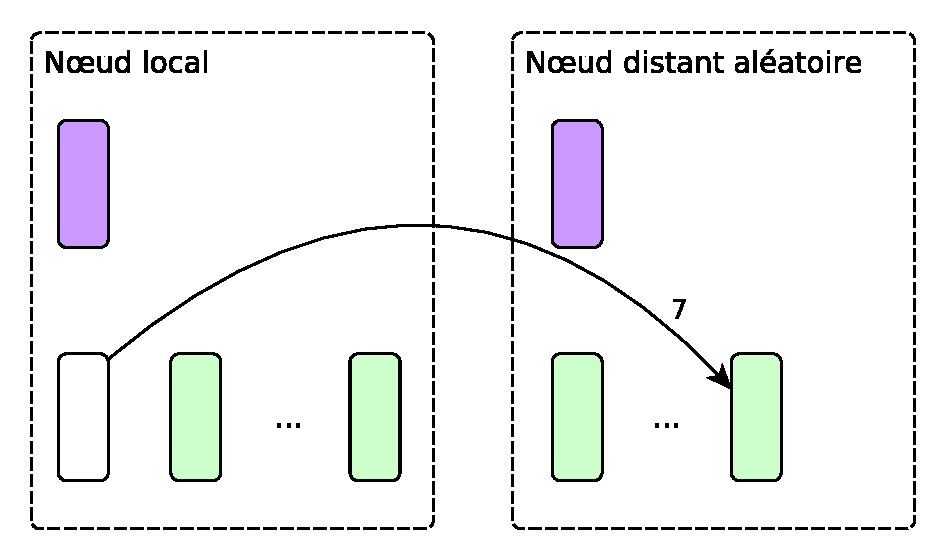
\includegraphics[width=0.6\textwidth]{graph/steal_strategies_anim_7.pdf}%
  }%
\end{figure}

\end{frame}

\begin{frame}
\frametitle{Éléments de comparaison}

Deux supports exécutifs grand public :

\begin{block}{libGOMP}
  \begin{itemize}
    \item Livré avec GCC
    \item Pas de vision hiérarchique de la machine
    \item Pas de vol de travail (algorithme glouton avec une queue centralisée)
  \end{itemize}
\end{block}

\begin{block}{libOMP}
  \begin{itemize}
    \item Livré avec Clang (Intel)
    \item Vol de travail classique (une queue par coeur)
    \item Sélection aléatoire, placement local
  \end{itemize}
\end{block}

\end{frame}




\begin{frame}
\frametitle{Matériel}

\begin{block}{Machine : idchire}
    \begin{itemize}
\item Intel Xeon E5-4640 @ 2.4 GHz, Sandy Bridge
\item 24 noeuds NUMA, 8 coeurs par noeud, 192 coeurs.
\item Cache L3 : 20 Mo
    \end{itemize}
\end{block}

\end{frame}

\begin{frame}
  \frametitle{Comparaison des supports exécutif}
  Cholesky, en fonction de la taille de matrice, sur idchire
  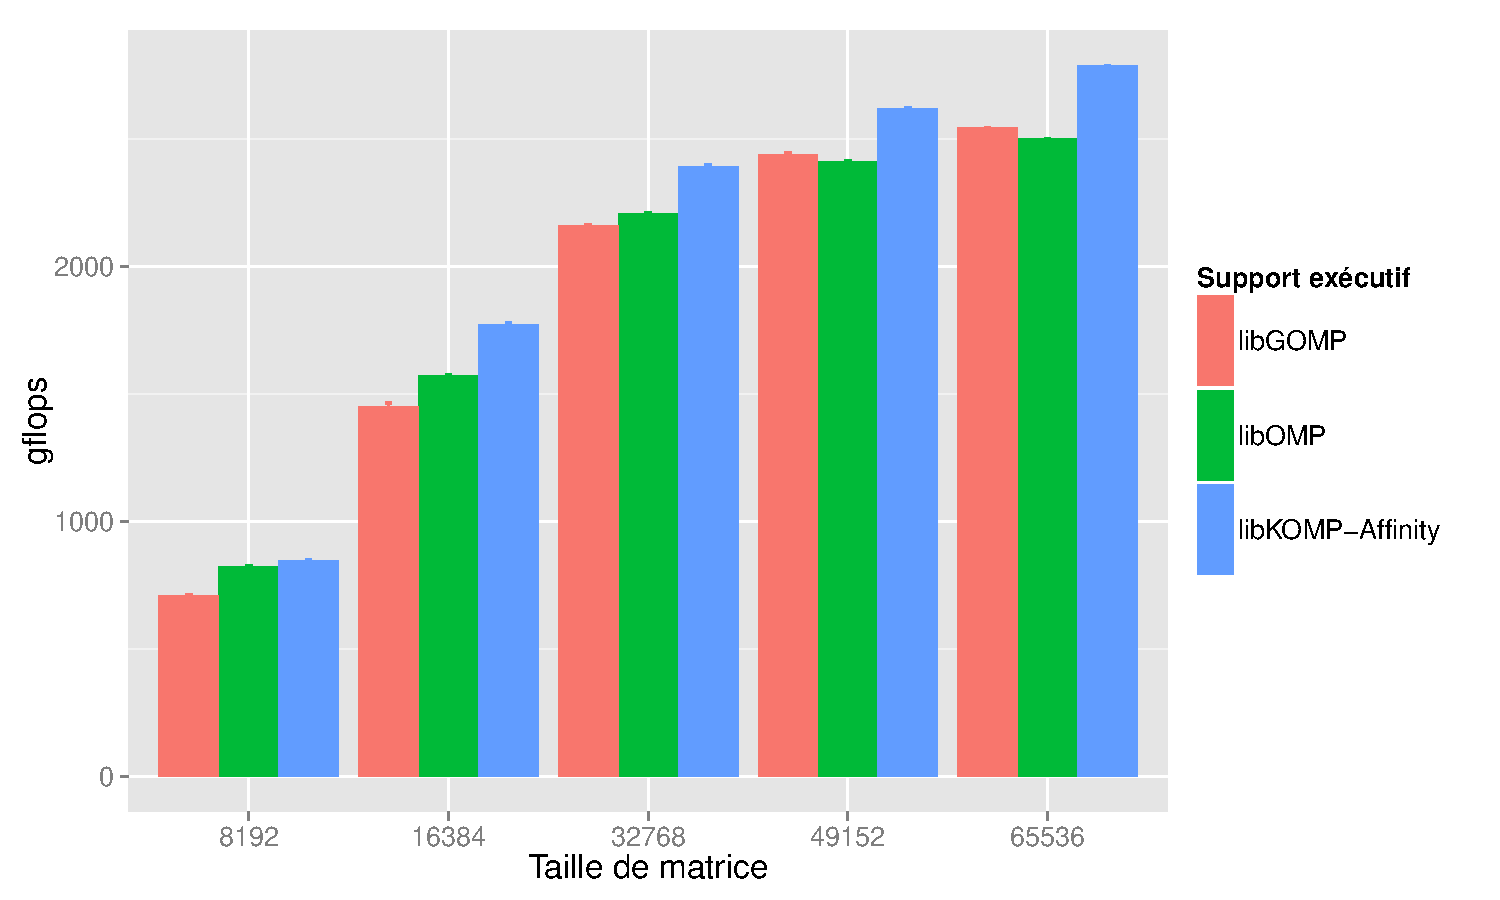
\includegraphics[width=0.9\textwidth]{graph/graph_details_cholesky_idchire.pdf}
\end{frame}

\begin{frame}
  \frametitle{Comparaison des supports exécutif}
  Évaluation sur deux tailles choisies
  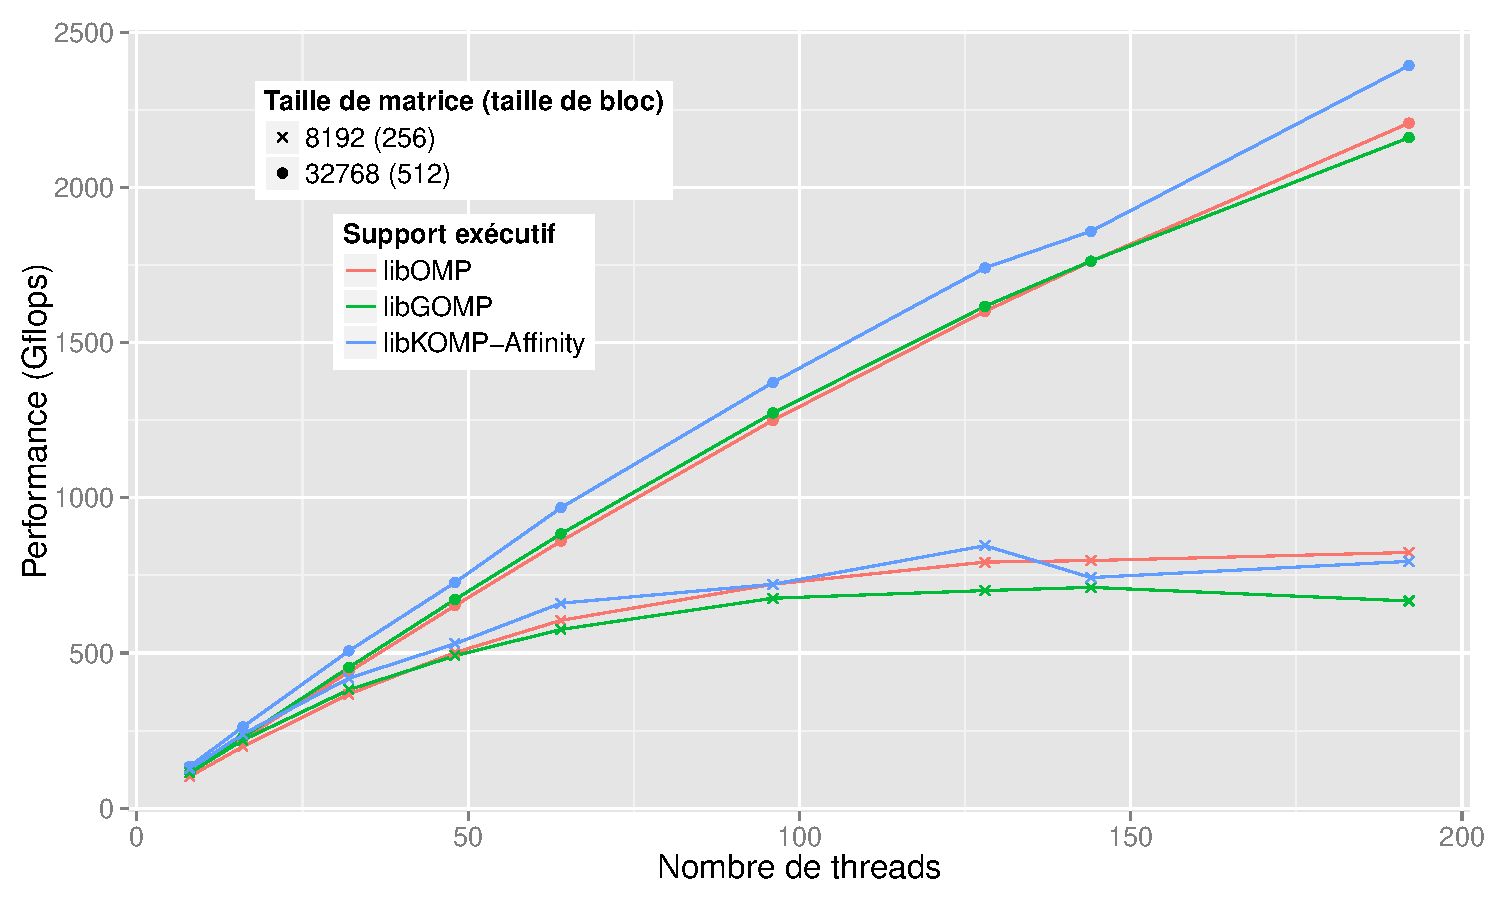
\includegraphics[width=0.9\textwidth]{graph/graph_all_cholesky_idchire.pdf}
\end{frame}

\begin{frame}
  \frametitle{Premières conclusions}
  \begin{exampleblock}{Améliorations}
    \begin{itemize}
      \item Différence visible dès l'utilisation de plusieurs noeuds NUMA
      \item Impact significatif pour les tailles de blocs importantes
    \end{itemize}
  \end{exampleblock}

  \begin{alertblock}{Limites}
    \begin{itemize}
      \item Peu d'intérêt pour les petites tailles de bloc.
      \item Machine "favorable" : 24 noeuds NUMA, avec un facteur NUMA important.
    \end{itemize}
  \end{alertblock}
\end{frame}

\begin{frame}
\frametitle{Deuxième machine}

\begin{block}{Machine : brunch}
  Plus récente, et topologie plus simple :
  \begin{itemize}
    \item Intel Xeon E7-8890 @ 2.2 GHz, Broadwell
    \item 4 noeuds NUMA, 24 coeurs par noeud, 96 coeurs
    \item Cache L3 : 60 Mo (similaire à idchire, 2.5 Mo par coeur)
  \end{itemize}
\end{block}

\end{frame}

\begin{frame}
  \frametitle{Comparaison des supports exécutif}
  Évaluation sur deux tailles choisies
  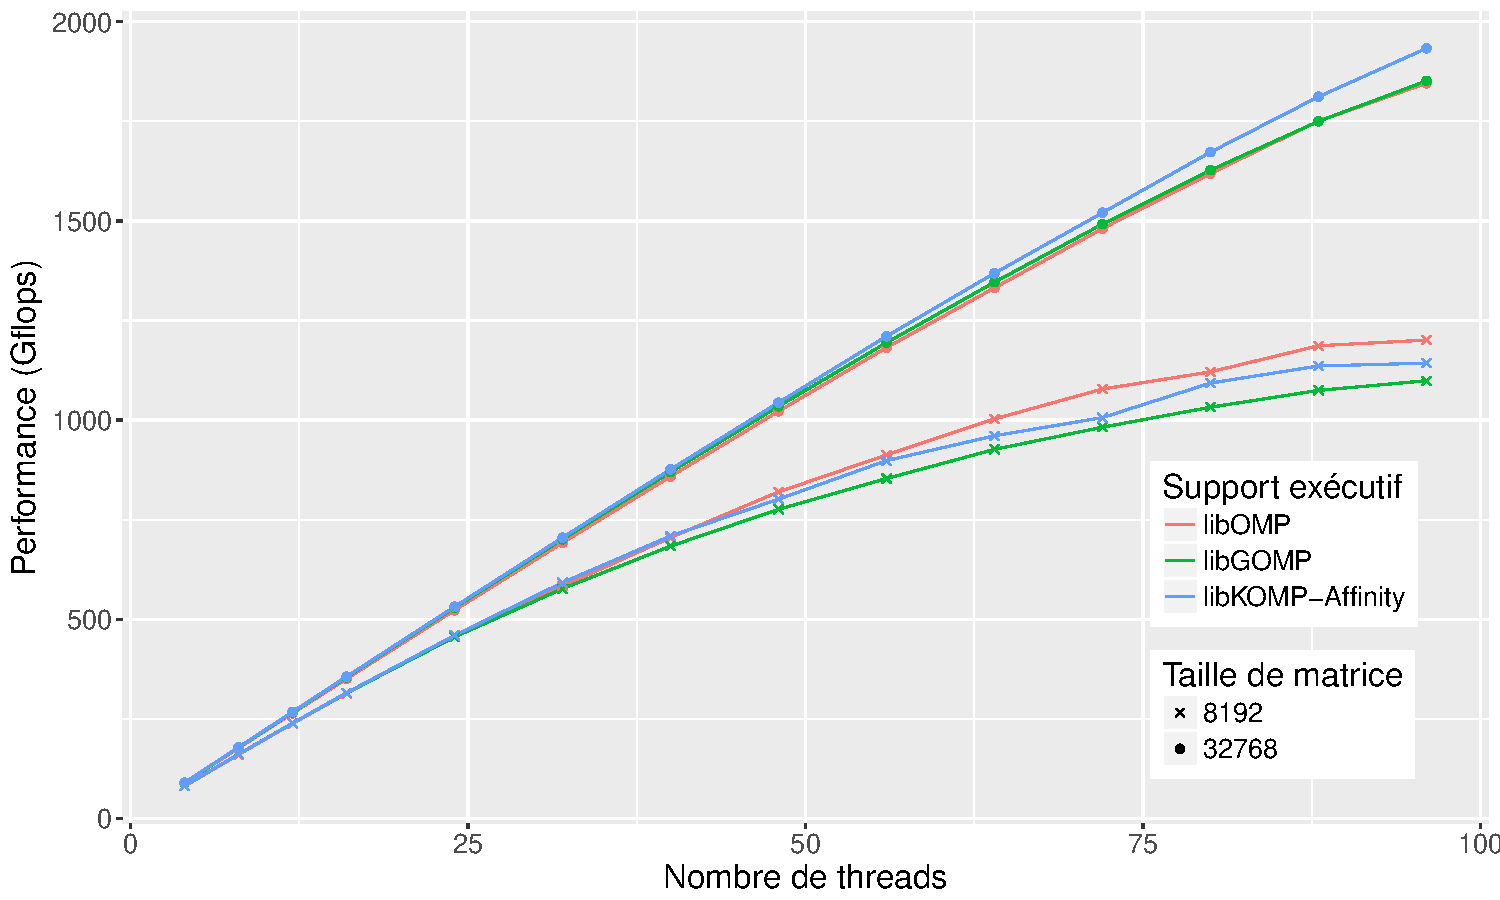
\includegraphics[width=0.9\textwidth]{graph/graph_all_cholesky_brunch.pdf}
\end{frame}

\begin{frame}
  \frametitle{Conclusions}

  \begin{block}{Différence de machine}
    \begin{itemize}
      \item Comportement similaire
      \item Impact absolu moindre (du à la topologie)
    \end{itemize}
  \end{block}

  \uncover<2>{
    \begin{block}{Intuition générale}
      Affinité assez simple à mettre en place, rentable lorsque les dataset manipulés par les tâches sortent du L3.
    \end{block}
  }
\end{frame}


\begin{frame}
  \frametitle{Plan}
  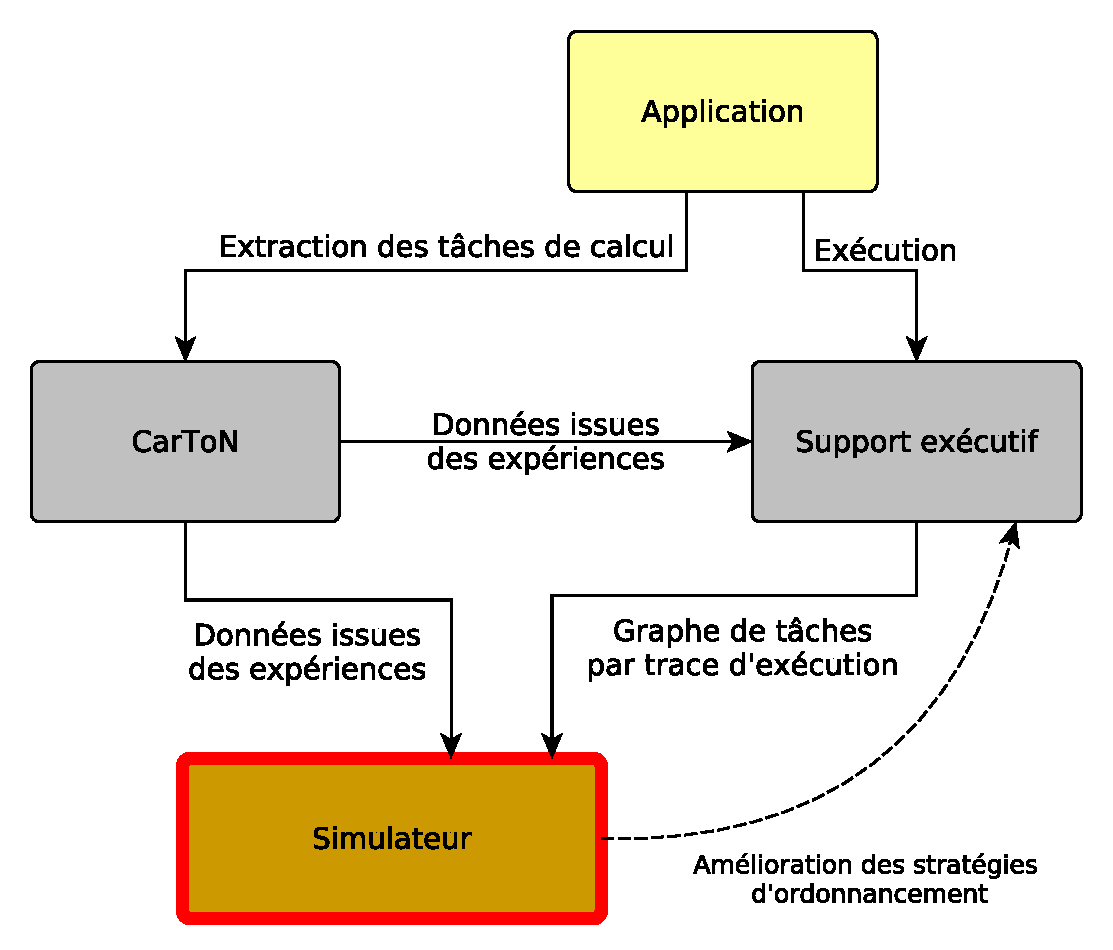
\includegraphics[width=0.8\textwidth]{graph/big_picture-part3.pdf}
\end{frame}


\begin{frame}[fragile]
  \frametitle{Motivation pour la simulation}

  \begin{itemize}
    \item Développer dans un support exécutif réel à un coût.

      Simulation => expérimentations et développement rapides

    \item Pouvoir prendre les meilleures décisions

      On a "le temps" pour les prendre

    \item Utilisation des caractéristiques des tâches

      Positionnement du support exécutif par rapport aux performances attendues.
  \end{itemize}


\end{frame}

\begin{frame}[fragile]
  \frametitle{Composants du simulateur}
  \begin{itemize}
    \item Données

      Blocs de taille fixe, associés à un noeud (\emph{first-touch})

    \item Tâches

      Décomposées en un ensemble d'action de trois types \verb/read/, \verb/write/, \verb/compute/

    \item Modèle d'exécution

      Vol de travail
  \end{itemize}

\end{frame}

\begin{frame}[fragile]
  \frametitle{Modélisation}

  Modèle de coût basique :

  \begin{itemize}
    \item Une tâche (\verb/read/+\verb/write/+\verb/compute/) = un coût unique
  \end{itemize}

  Coûts déterminés par les données de CarToN, en fonction du contexte d'exécution
  \begin{itemize}
    \item Accès local/distant
    \item Charge de la machine
  \end{itemize}

\end{frame}

\begin{frame}
  \frametitle{Stratégies et modèles considérés}

  \begin{block}{Vol de travail}
    Stratégies similaires à celles implémentées dans le support exécutif :
    \begin{itemize}
      \item Aléatoire
      \item Hiérarchique avec affinité.
    \end{itemize}
  \end{block}

  \begin{block}{Coûts des tâches}
    \begin{itemize}
      \item Maximum : meilleure performance observée de la tâche
      \item Distant : moins bonne performance distante observée
      \item Deux niveaux : utilisation du contexte d'exécution pour choisir le coût adapté
    \end{itemize}
  \end{block}

  Objectif : essayer de borner l'exécution réelle.
\end{frame}


\begin{frame}
  \frametitle{Évaluation}
  Matrice N=32768, BS=512 (~45000 tâches)
  \begin{figure}
    \only<1>{%
      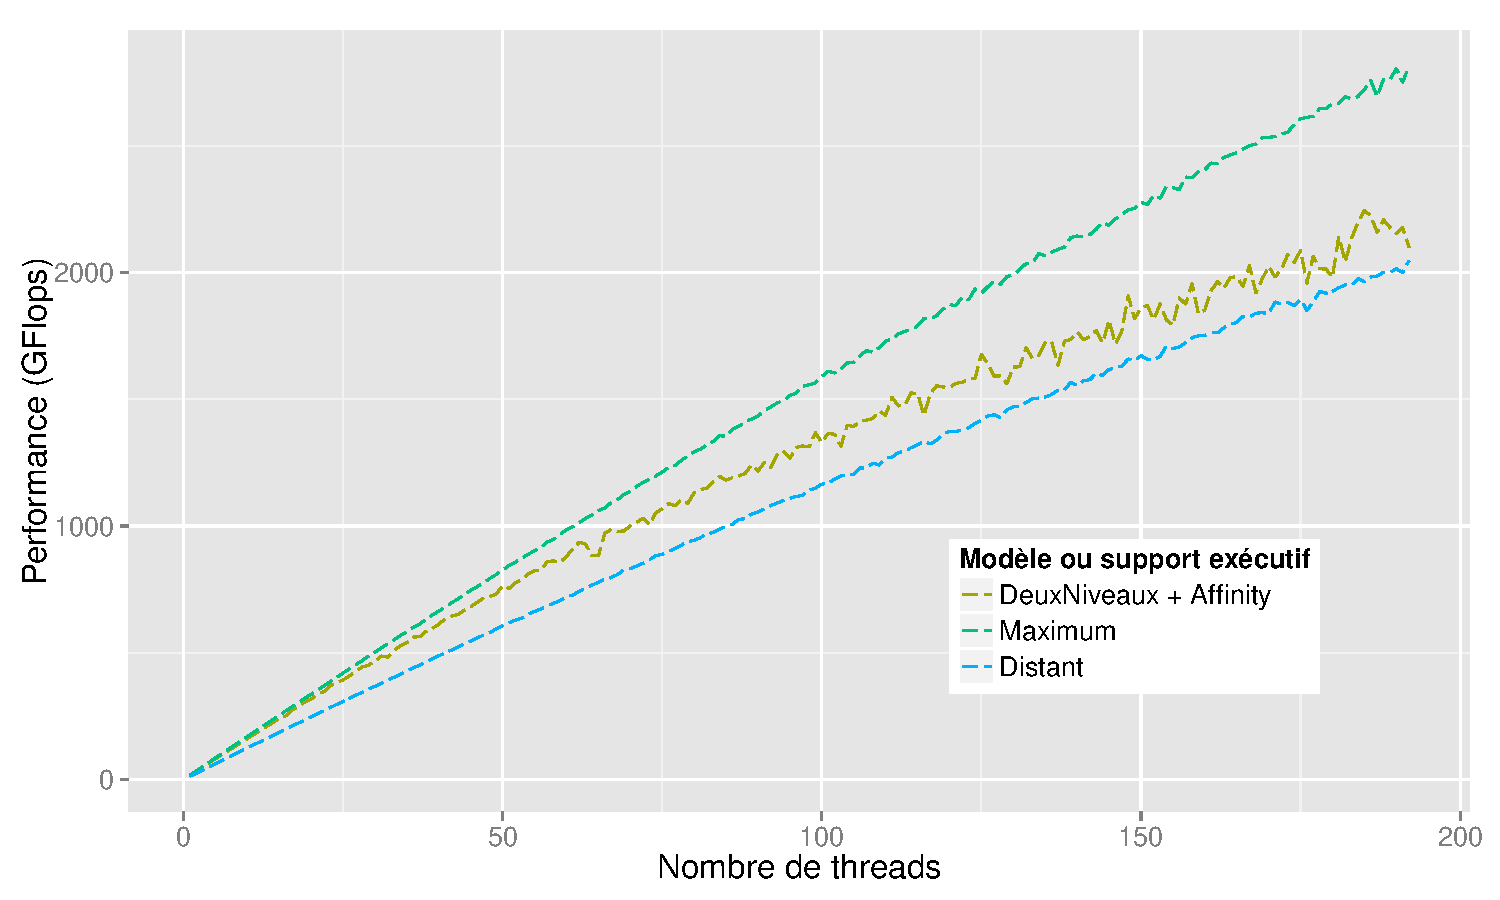
\includegraphics[width=\textwidth]{graph/simu_affinity_runtime_idchire_0.pdf}%
    }%
    \only<2>{%
      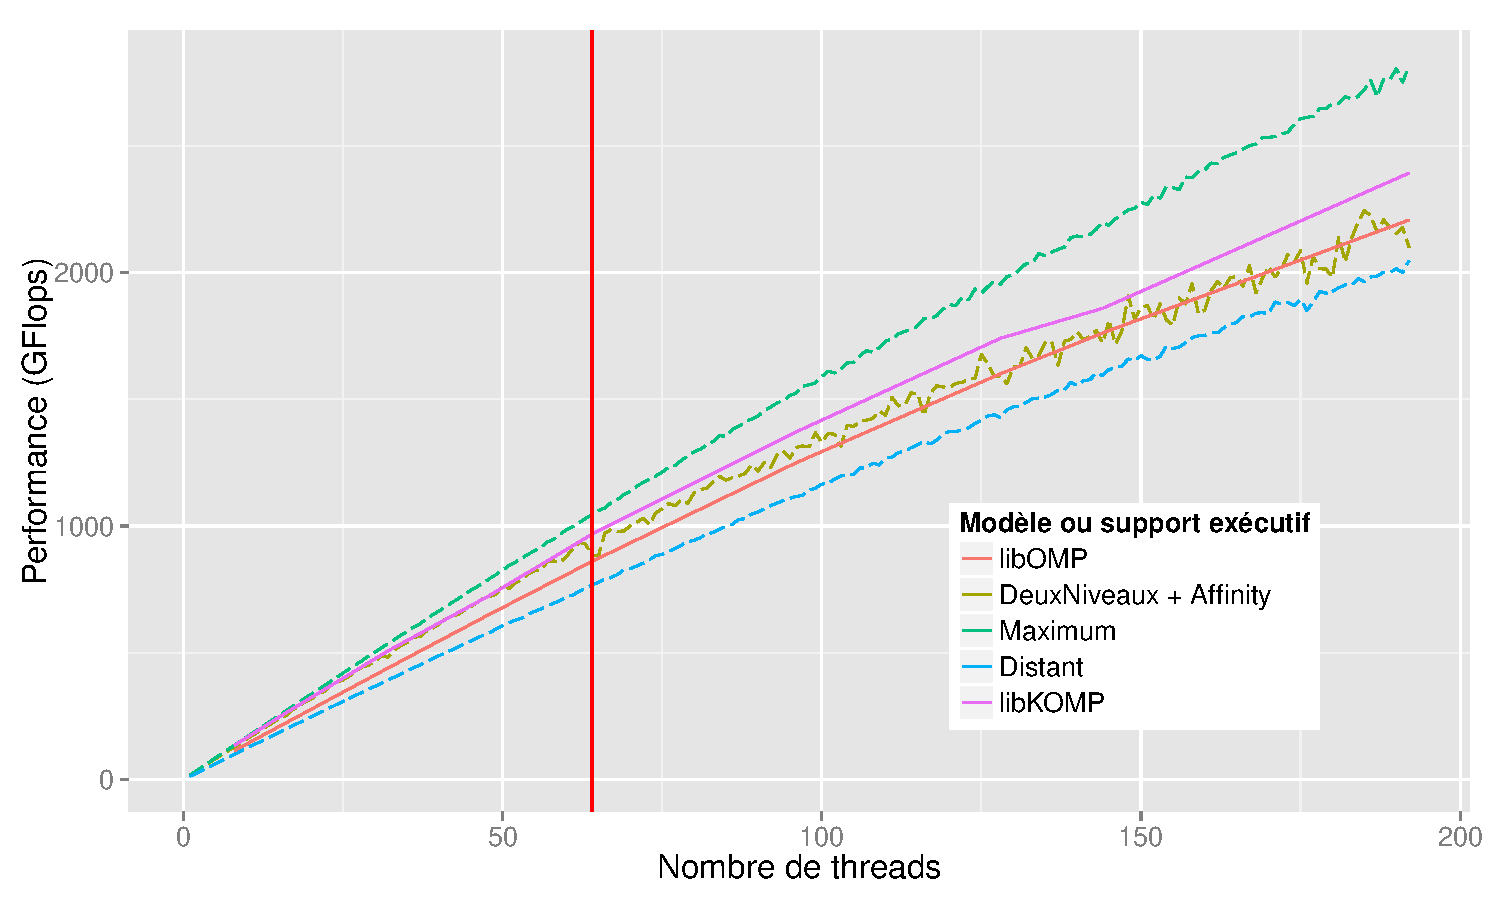
\includegraphics[width=\textwidth]{graph/simu_affinity_runtime_idchire.pdf}%
    }%
  \end{figure}


\end{frame}

\begin{frame}
  \frametitle{Évaluation}
  Matrice N=8192, BS=256 (~6000 tâches)
  \begin{figure}
    \only<1>{%
      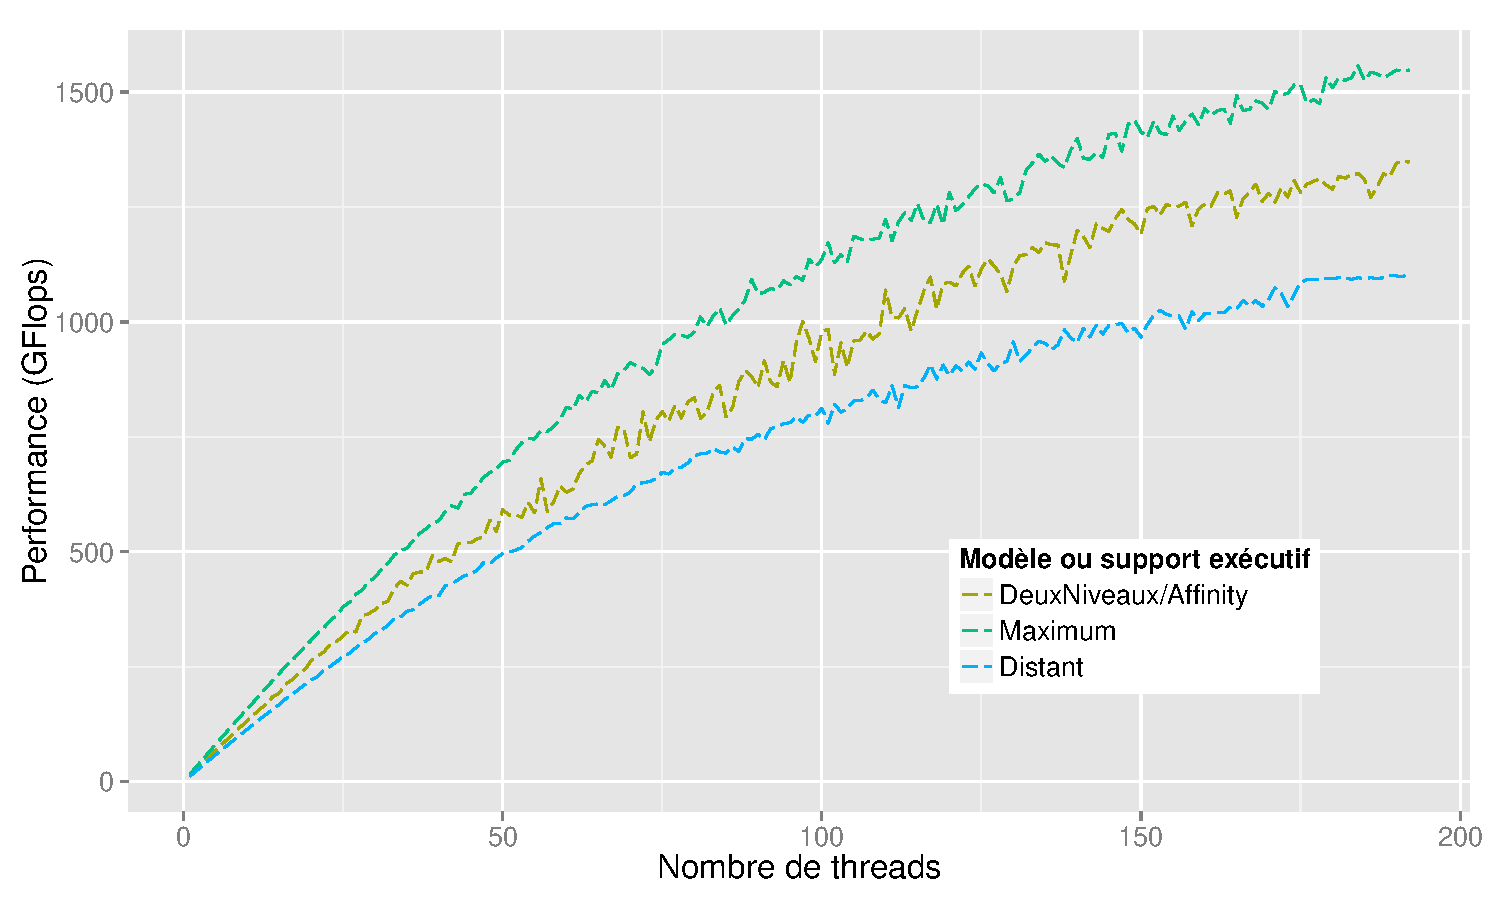
\includegraphics[width=\textwidth]{graph/simu_affinity_8k_runtime_idchire_0.pdf}%
    }%
    \only<2>{%
      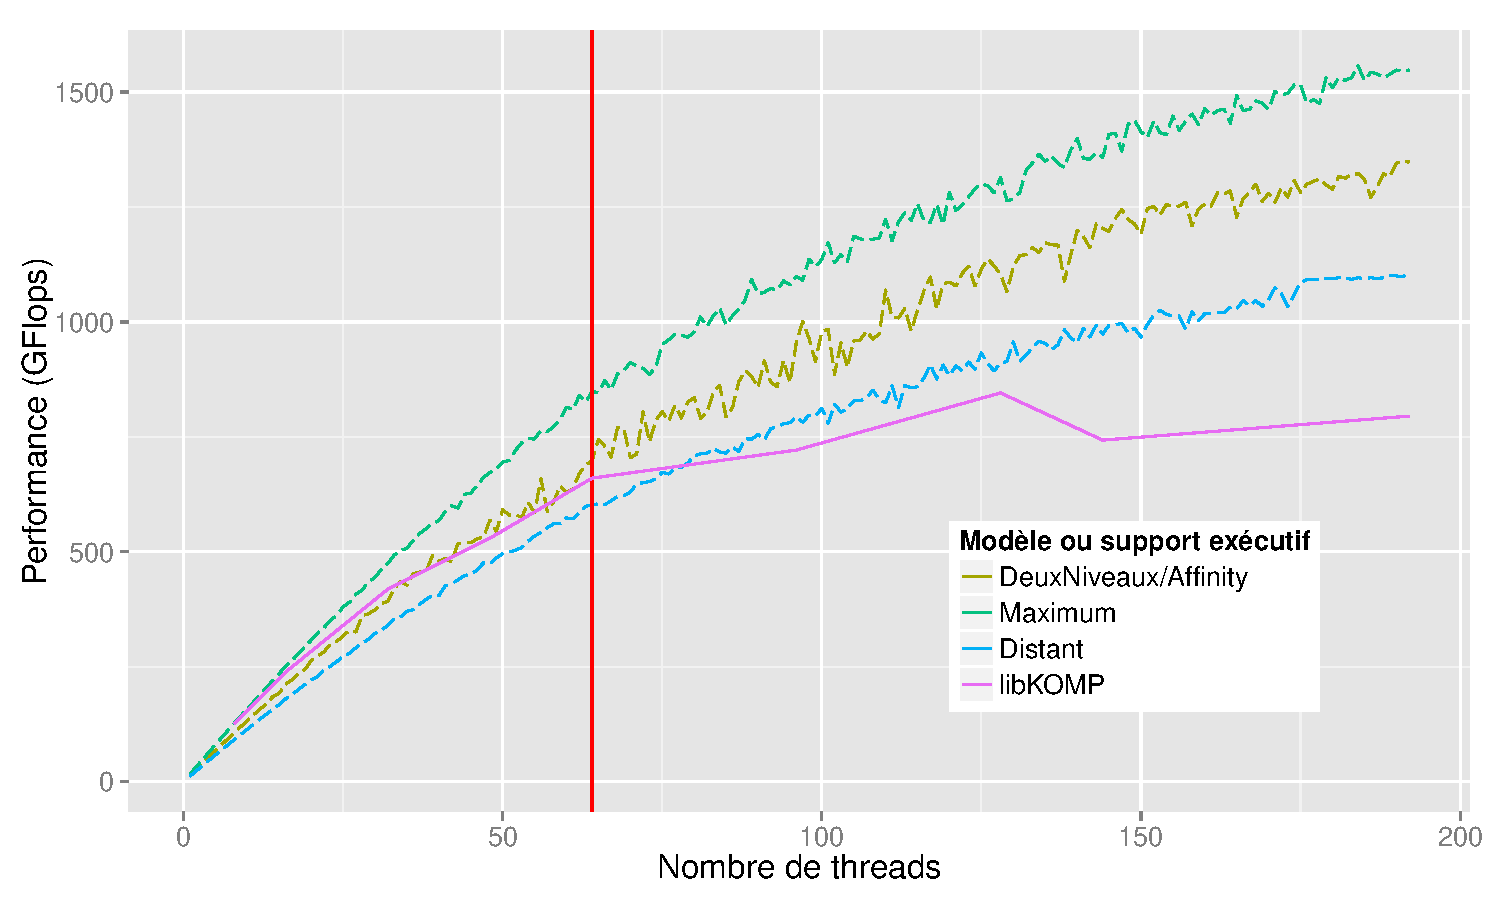
\includegraphics[width=\textwidth]{graph/simu_affinity_8k_runtime_idchire.pdf}%
    }%
  \end{figure}


\end{frame}


\begin{frame}
  \frametitle{Discussions}

  \begin{block}{Conclusion des premières expériences}
    \begin{itemize}
      \item Résultat assez réaliste compte tenu de l'existant
      \item Bémol sur les cas à "faible" parallélisme
    \end{itemize}
  \end{block}
  \begin{block}{Perspectives}
    \begin{itemize}
      \item Utilisation de coûts plus précis
      \item Modélisation de la machine (caches, bande passante)
      \item Amélioration des distributions de données
    \end{itemize}
  \end{block}
\end{frame}

\begin{frame}
  \frametitle{Synthèse}

    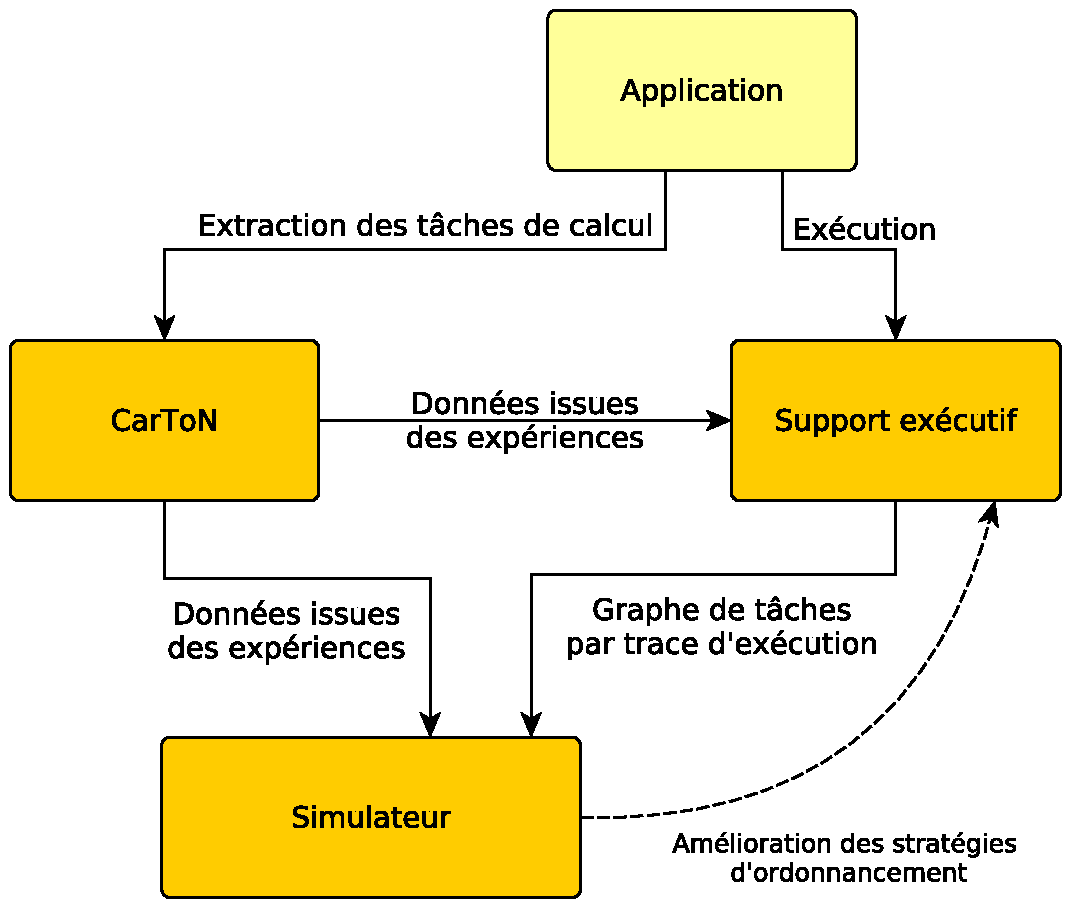
\includegraphics[width=\textwidth]{graph/big_picture.pdf}
  %\begin{block}{Processus complet pour une application}
    %\begin{itemize}
      %\item Observations générales et détaillées de l'application
      %\item Exécution prenant en compte les caractéristiques importantes
      %\item Ajustement des heuristiques d'ordonnancement via simulateur
    %\end{itemize}
  %\end{block}
\end{frame}


\begin{frame}
  \frametitle{Perspectives de la thèse}

  TODO

\end{frame}


%\begin{frame}[fragile]
%\frametitle{Exemples d'applications par tâches}
%\begin{columns}[T,onlytextwidth]
  %\column{0.5\textwidth}
%\begin{onlyenv}<1>
  %\small{extrait d'un Jacobi (Stencil) :}
  %\begin{lstlisting}[numbers=none]
%for (int j = 0; j < ny; j += block_size) {
  %for (int i = 0; i < nx; i += block_size) {
    %/*... compute neighbors ...*/
%#pragma omp task
    %shared(/*...*/)
    %firstprivate(/*...*/) \
    %depend(out: unew[i][j]) \
    %depend(in: f[i][j], \
               %u[i][j], \
               %u[(i - xdm1)][j], \
               %u[i][(j + ydp1)], \
               %u[i][(j - ydm1)], \
               %u[(i + xdp1)][j])
    %compute_estimate(f, u, unew, /*...*/);
  %}
%}
%\end{lstlisting}

%\end{onlyenv}
  %\column{0.45\textwidth}
  %\small{extrait de Cholesky (Algèbre linéaire):}

%\begin{lstlisting}[numbers=none]
%/*...*/
%for (n = k+1; n < m; n++) {
%#pragma omp task depend(in:dA[k][n],
                           %dB[k][m])
                 %depend(inout:dC[n][m]])
    %cblas_dgemm(dA, dB, dC, /*...*/);
%}
%/*...*/
%\end{lstlisting}
%\end{columns}

%\uncover<2>{
%\begin{tikzpicture}[overlay, remember picture]
%\node[anchor=south west] (img2) at (1, -2) {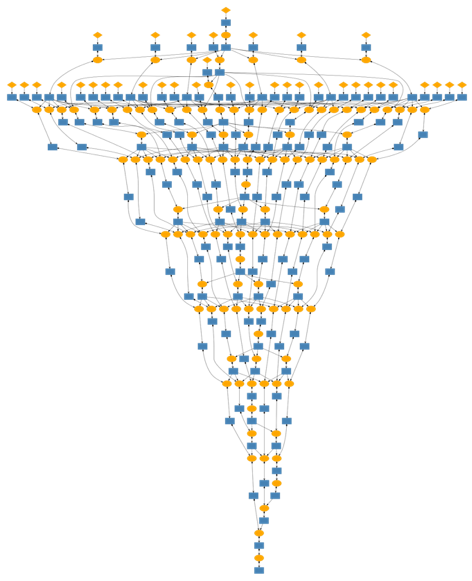
\includegraphics[width=0.4\textwidth]{graph/dfg_depotrf.png}};
    %\end{tikzpicture}
%}
%\end{frame}



%\begin{frame}
%\frametitle{Motivations}

%\begin{figure}
  %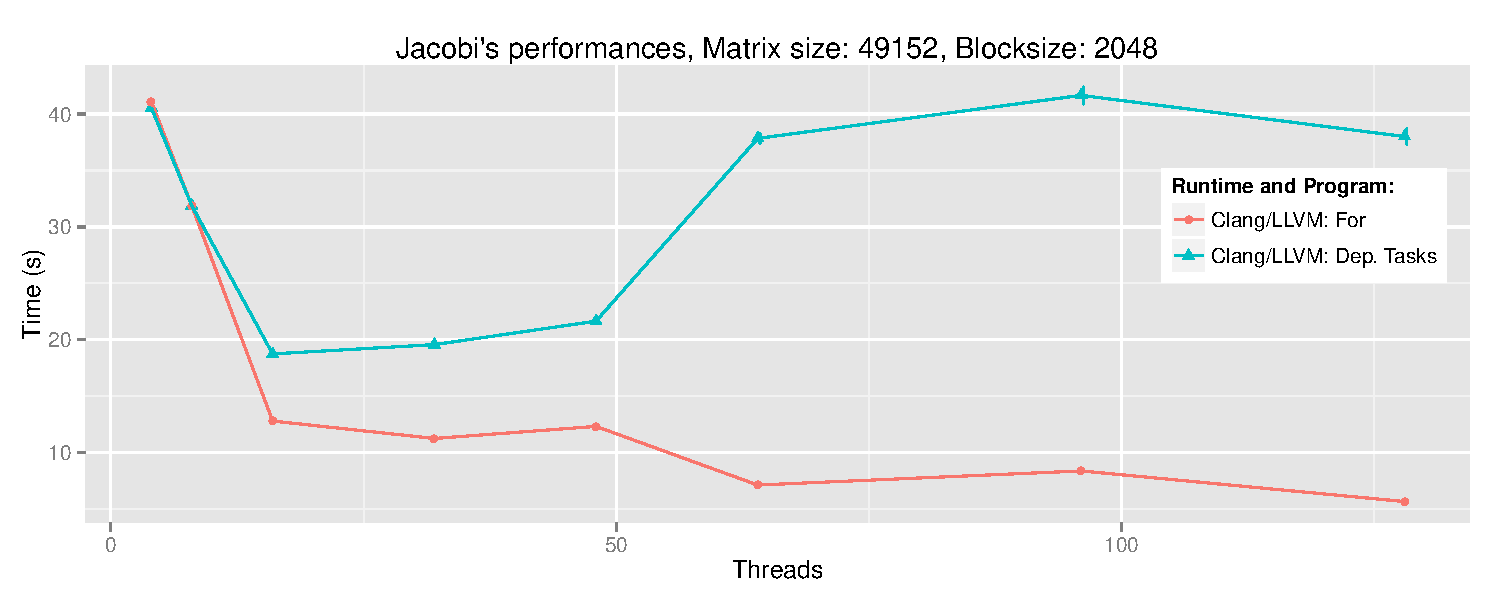
\includegraphics[width=\textwidth]{./graph/jacobi_scale_iomp.pdf}
%\end{figure}

%\begin{alertblock}{Cause principale}
  %pas de localité temporelle dans la version avec tâches !
%\end{alertblock}
%\end{frame}



%\begin{frame}
%\frametitle{Applications et machines}

%\begin{block}{Suite de benchmarks KASTORS}
  %Applications utilisées :
  %\begin{itemize}
    %\item Algèbre linéaire (\textbf{Cholesky (dpotrf)}, QR, LU)
    %\item Stencil (Jacobi 2D)
  %\end{itemize}
%\end{block}

%\begin{block}{Machine : idchire}
    %\begin{itemize}
%\item Intel Xeon E5-4640 @ 2.4 GHz, Sandy Bridge
%\item 24 NUMA nodes, 8 cores per node, 192 total cores
    %\end{itemize}
%\end{block}

%\begin{block}{Logiciels}
  %Clang 3.9 + libKOMP (https://gitlab.inria.fr/openmp/libkomp/)
%\end{block}

%\end{frame}

%\begin{frame}
  %\frametitle{Étude de Cholesky}
  %\begin{center}
    %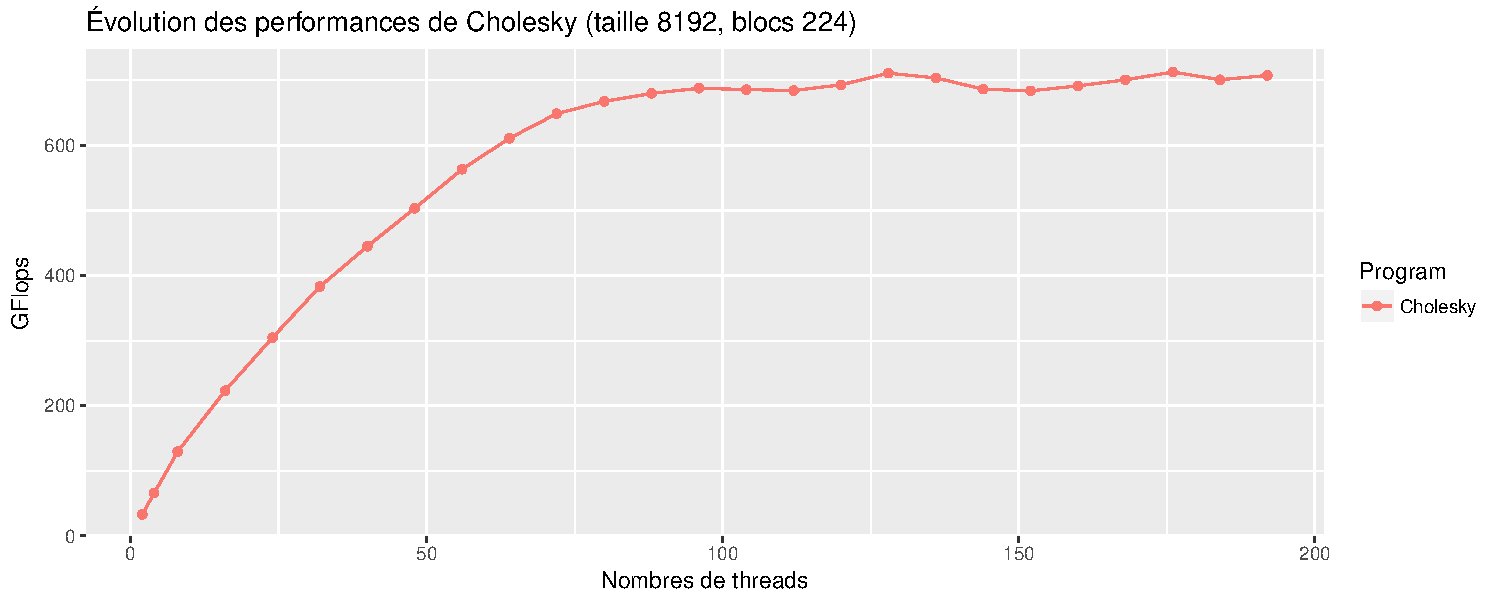
\includegraphics[width=\textwidth]{./graph/graph_evolution_cholesky.pdf}
  %\end{center}
%\end{frame}

%\begin{frame}
  %\frametitle{Prédiction}

  %\begin{block}{Quid de la prédiction ?}
    %Discussions avec Julien Langou (UC Denver) :
    %\begin{itemize}
      %\item Quelle(s) borne(s) sup théorique ?
      %\item Comment les améliorer ?
      %\item Distance des expériences vis à vis de la théorie ?
    %\end{itemize}
    
  %\end{block}
%\end{frame}

%\begin{frame}
  %\frametitle{Prédiction}
  %\begin{center}
    %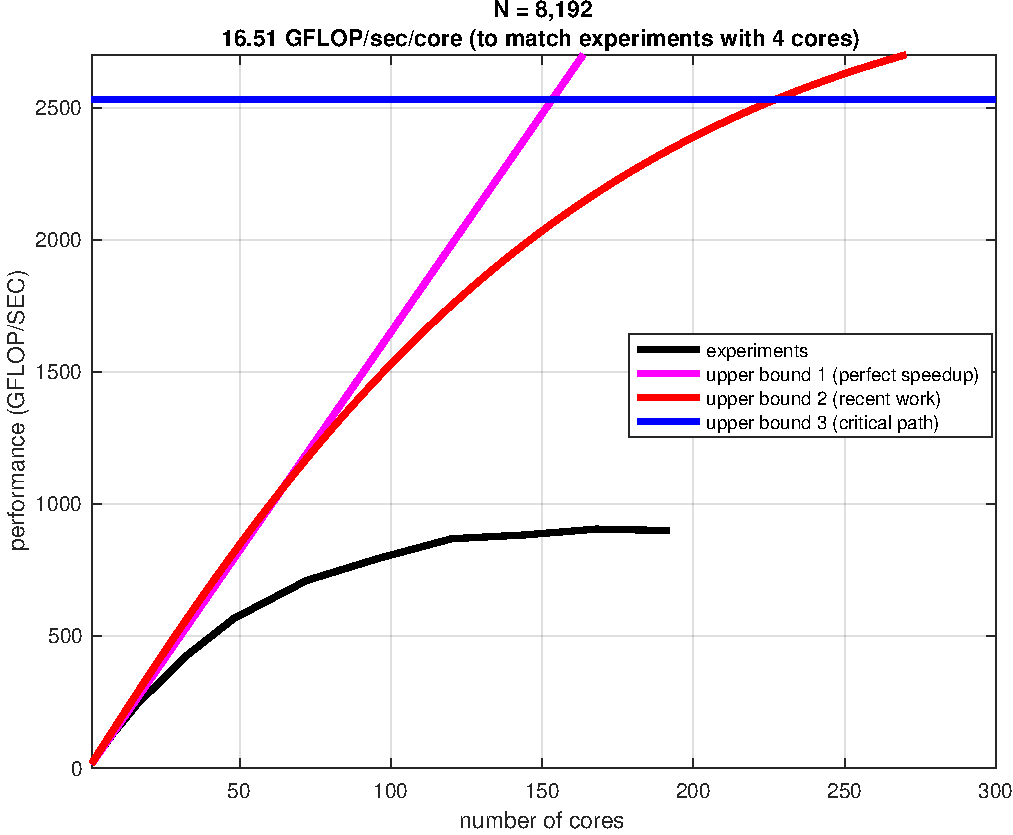
\includegraphics[width=0.7\textwidth]{./graph/julien_upperbound_v1.pdf}
  %\end{center}
%\end{frame}

%\begin{frame}
  %\frametitle{Oops !}
  %\begin{alertblock}{Grosse divergence sur la courbe !}
    %\begin{itemize}
      %\item Le support exécutif est mauvais ?
      %\item Le modèle *théorique* mauvais ?
    %\end{itemize}
  %\end{alertblock}
%\end{frame}

%\begin{frame}
  %\frametitle{Observations}
  %\begin{block}{Observations}
    %\begin{itemize}
      %\item Pour un nombre de threads donné, temps des noyaux variables
      %\item Quelques "îlots" dans la distribution
    %\end{itemize}
  %\end{block}
%\end{frame}



%\begin{frame}
  %\frametitle{Évolution du temps des noyaux}
  %\begin{center}
    %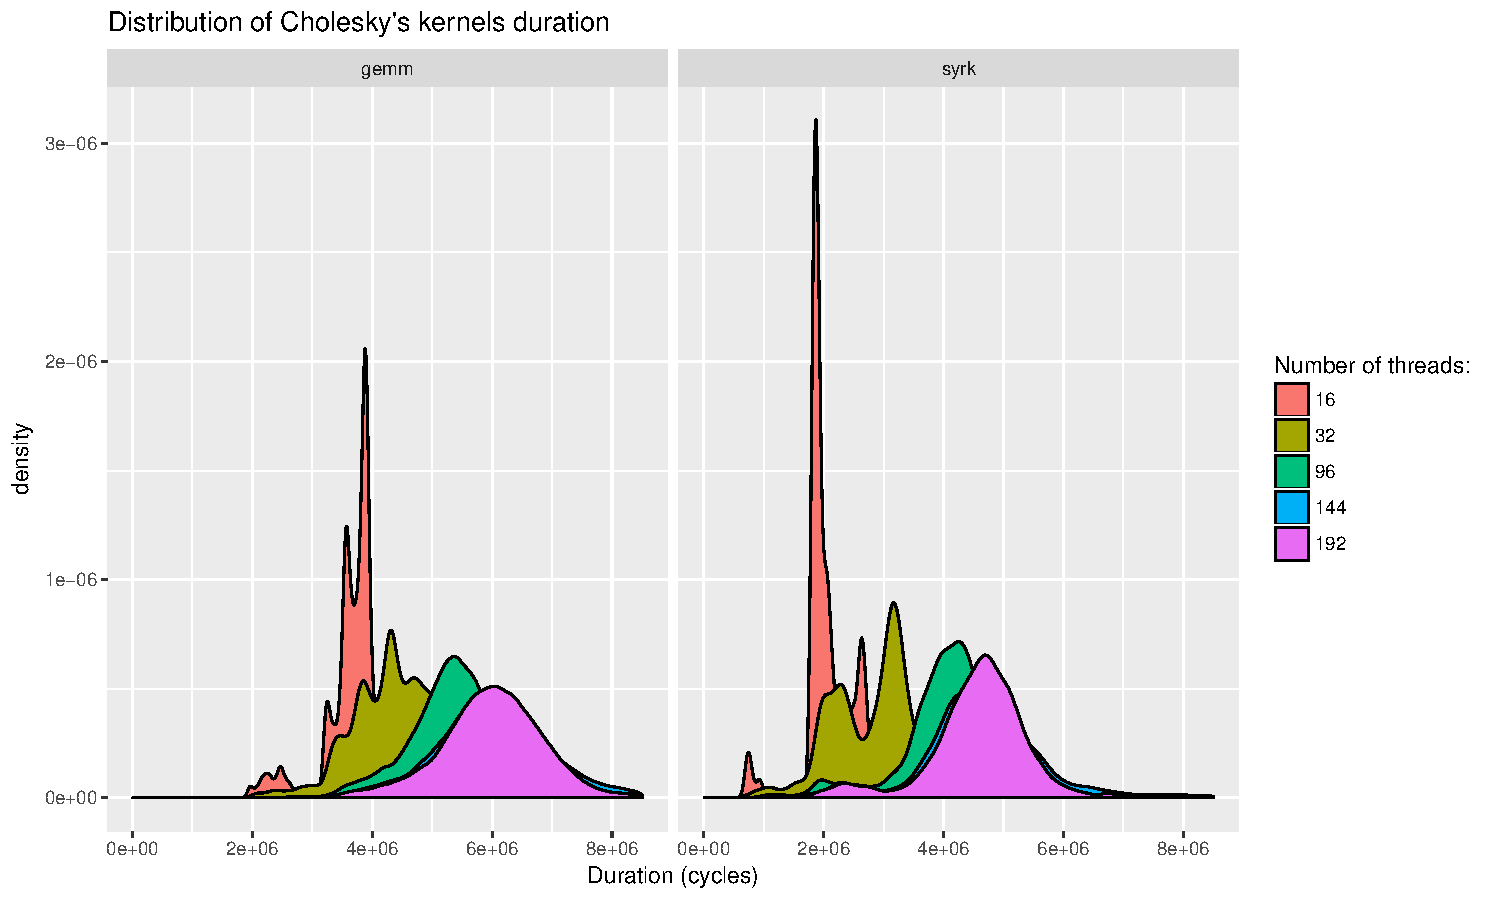
\includegraphics[width=0.8\textwidth]{graph/cholesky_kernel_evolution.pdf}
  %\end{center}
%\end{frame}

%\begin{frame}
  %\frametitle{Prédiction}
  %% courbe bleue : critical path, revisité via perf max par coeur
  %% courbe rouge : upper bound, revisité via perf max par coeur
  %\begin{center}
    %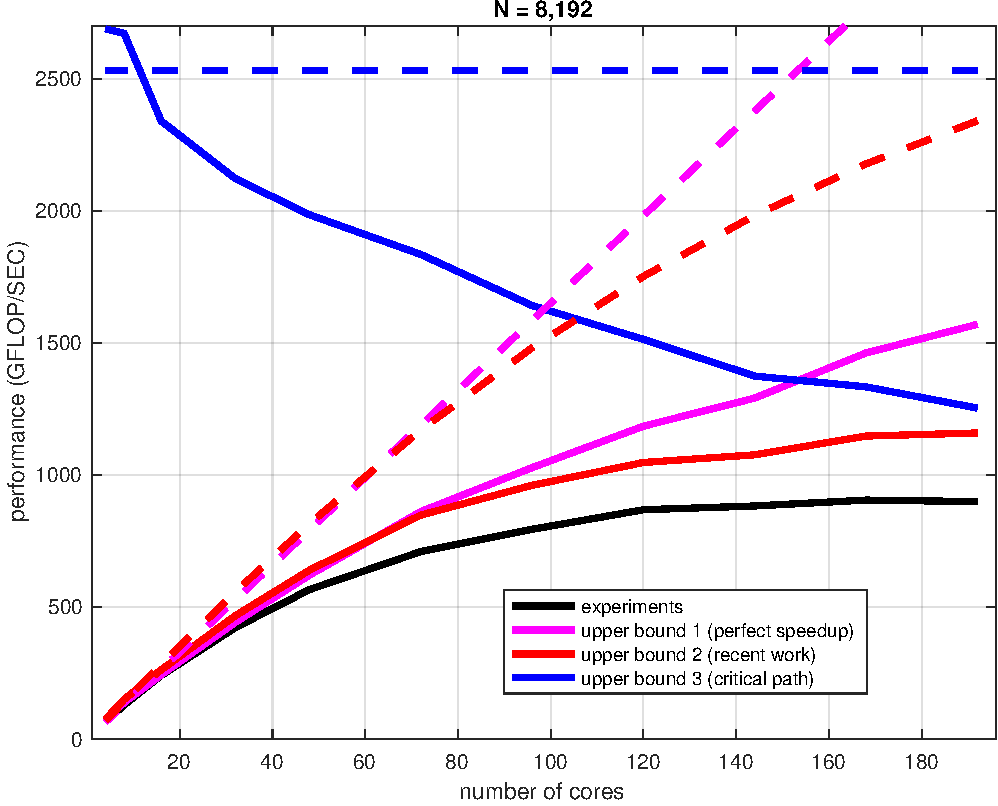
\includegraphics[width=0.7\textwidth]{./graph/julien_upperbounds_v2.pdf}
  %\end{center}
%\end{frame}

%\begin{frame}
  %\frametitle{Vers une convergence}
  %\begin{block}{Première conclusion}
    %Le modèle théorique était trop optimiste
  %\end{block}
  %\begin{exampleblock}{Meilleure cohérence}
    %\begin{itemize}
      %\item Critical path mis à jour
      %\item Upper bound mis à jour
    %\end{itemize}
    %=> Baisse des limites théoriquement atteignables
  %\end{exampleblock}
  %\begin{block}{Aller plus loin}
    %\begin{itemize}
      %\item Il "manque" 250 Glops...
      %\item Comment identifier les facteurs de ces variations ?
    %\end{itemize}
  %\end{block}
%\end{frame}



%\begin{frame}[fragile]
%\frametitle{Faciliter les expériences à l'aide d'un outil}

    %Fournir un moyen simple et fiable pour les utilisateurs d'exécuter des noyaux, avec un contrôle précis sur le placement physique des données et sur l'exécution des noyaux.

  %\begin{block}{L'utilisateur fourni}
    %\begin{itemize}
      %\item Des noyaux et données.
      %\item Des scenario : quoi allouer, où et quand ; quoi lancer, où et quand.
      %\item Des indicateurs à observer (temps, compteurs de perf, ...)
    %\end{itemize}
  %\end{block}

  %\begin{block}{L'outil garanti}
    %\begin{itemize}
      %\item Une exécution fiable du scenario sur l'architecture cible.

      %\item Pas de surcoût = observation uniquement du comportement des noyaux.
    %\end{itemize}
  %\end{block}

%\end{frame}


%\begin{frame}[fragile]
%\frametitle{Fonctionnement}
%\noindent{%
%\begin{minipage}[t]{0.48\linewidth}
  %\begin{block}{"Support exécutif"}
    %\begin{itemize}
      %\item Un thread par coeur (pinned)
      %\item Noyaux empilés par coeur
      %\item Synchronisation si besoin
      %\item Relève des indicateurs avant/après
    %\end{itemize}
  %\end{block}
  %\begin{block}{Exemples}
    %\begin{itemize}
      %\uncover<2->{
        %\only<2>{
          %\item {\color{red}Données}
        %}
        %\only<3-4>{
          %\item Données
        %}
      %}
      %\uncover<3->{
	%\only<3>{
		%\item {\color{red}Actions}
	%}
	%\only<4>{
		%\item Actions
	%}
      %}
      %\uncover<4->{
        %\item {\color{red}Indicateurs}
      %}
    %\end{itemize}
  %\end{block}
%\end{minipage}}%
%\hfill%
%\begin{minipage}[t]{0.48\linewidth}

  %\begin{onlyenv}<2>
  %\begin{lstlisting}[numbers=none,language=yaml]
%scenario:
  %# ...
  %data:
    %- a:
      %- type: "double *"
    %- b:
      %- type: "double *"
    %- c:
      %- type: "double *"
    %- block_size:
      %- type: "int"
      %- value: 256
  %# ...
%\end{lstlisting}
  %\end{onlyenv}
  %\begin{onlyenv}<3>
  %\begin{lstlisting}[numbers=none,language=yaml]
%scenario:
  %# ...
  %actions:
    %- kernel: init_blas_bloc
      %sync: false
      %params: 
      %- a
      %- block_size
      %core: 0
      %repeat: 1
    %- kernel: dgemm
      %sync: false
      %params: 
      %- a
      %- b
      %- c
      %- block_size
      %core: 0
      %repeat: 50
%\end{lstlisting}
  %\end{onlyenv}
  %\begin{onlyenv}<4>
  %\begin{lstlisting}[numbers=none,language=yaml]
%scenario:
  %# ...
  %watchers:
    %flops_dgemm:
      %- block_size
    %papi:
      %- PAPI_TOT_CYC
      %- PAPI_L3_TCM
%\end{lstlisting}
  %\end{onlyenv}
%\end{minipage}

%\end{frame}
%\begin{frame}
  %\frametitle{Scenario simple d'oservation des dgemm}
  %\begin{block}{dgemm}
    %Multiplication de matrice : C = A*B + C
    %\begin{itemize}
      %\item Dominant dans Cholesky !
      %\item A et B : lu
      %\item C : lu et écrit
    %\end{itemize}
  %\end{block}

  %\begin{block}{Scenario}
    %\begin{itemize}
      %\item Matrices carrées (..., 256, 512, ...)
      %\item Allocation des données sur le nœud local, ou un nœud distant
      %\item Exécution simultanée de 50 dgemm indépendants sur N cœurs (1->192)
      %\item Observation des GFlops.
    %\end{itemize}
  %\end{block}


%\end{frame}

%\begin{frame}
  %\frametitle{Résultats synthétiques}
  %\begin{center}
    %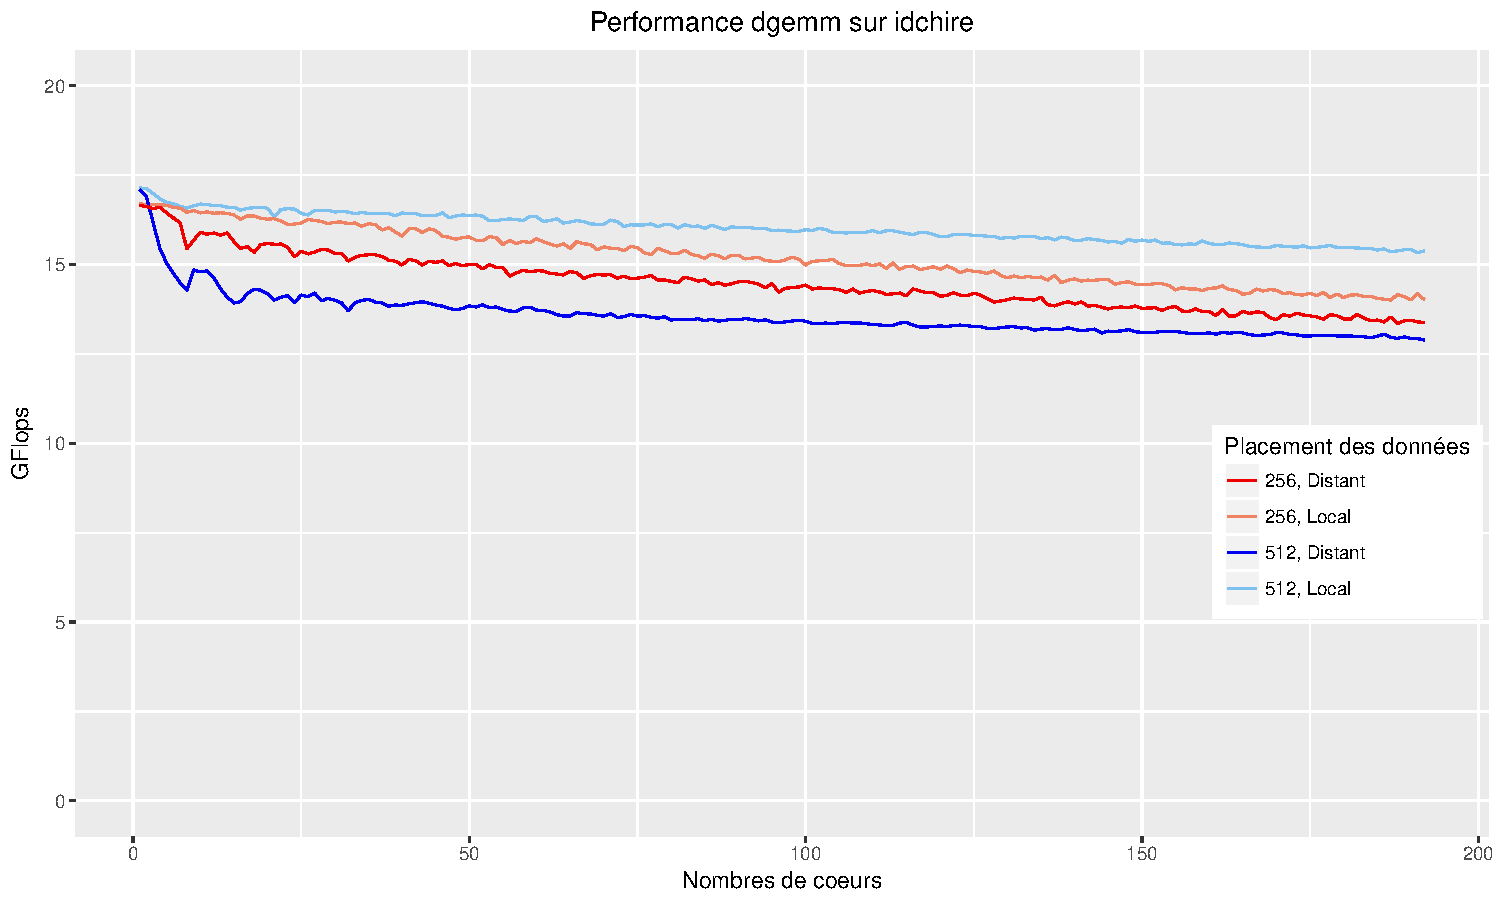
\includegraphics[width=\textwidth]{./graph/dgemm_local_vs_remote.pdf}
  %\end{center}

%\end{frame}
%\begin{frame}[fragile]
%\frametitle{What information does it have?}


        %\begin{lstlisting}
%void foo(double *a, size\_t blocksize) {
  %#pragma omp parallel num_threads(3)
  %{
    %#pragma omp task depend(out:a[0:blocksize])
      %write_on(a);
    %#pragma omp task depend(in:a[0:blocksize])
      %display(a);
  %}
%}
        %\end{lstlisting}
%\noindent{%
%\begin{minipage}[t]{0.48\linewidth}
  %\begin{block}{Available:}
    %\begin{itemize}
      %\item DAG
      %\item Size of data manipulated
      %\item Operations done on the data
    %\end{itemize}
  %\end{block}
%\end{minipage}}%
%\hfill%
%\begin{minipage}[t]{0.48\linewidth}
  %\begin{block}{Deducible:}
    %\begin{itemize}
      %\item Data placement on the architecture
      %\item "Importance" of a task
    %\end{itemize}
  %\end{block}
%\end{minipage}


%\end{frame}



%\begin{frame}[fragile]
%\frametitle{Moyens actuels de contrôler l'affinité}

%\begin{block}{Affinité pour les threads}
  %\begin{itemize}
    %\item Définir des \verb/places/ (à travers \verb/OMP_PLACES/)
    %\item Utiliser \verb/proc_bind/ pour utiliser une politique de placement des threads spécifique
  %\end{itemize}
%\end{block}

%\begin{block}{Affinité entre une tâche et une donnée ?}
  %\begin{itemize}
    %\item Allocation mémoire \verb/first-touch/ (plupart des Linux)
    %\item Librairies spécifiques à l'allocation de données
  %\end{itemize}
  %Pas (encore) de support dans le standard
%\end{block}

%\end{frame}

%\begin{frame}[fragile]
%\frametitle{Approaches}

  %\begin{block}{Programmer's point of view}
    %\begin{itemize}
      %\item OpenMP compiler's extension

        %\verb/affinity/ between a task and its data (core/NUMA node level)
    %\end{itemize}
  %\end{block}

  %\begin{block}{Runtime's point of view}
    %\begin{itemize}
      %\item Hierarchical workstealing
      %\item Locality-aware schedulers (based on programmer hints, or dep information)
    %\end{itemize}
  %\end{block}

%\end{frame}


%\begin{frame}[fragile]
%\frametitle{Approches en discussion}

%\begin{block}{Clause affinité pour les tâches}
%Exprimer une affinité entre une tâche et "quelque chose" sur la machine
  %\begin{itemize}
    %\item Thread

      %\textcolor{YellowOrange}{
      %Cette tâche devrait être exécutée près de ce thread
    %}
    %\item Donnée

      %\textcolor{YellowOrange}{
      %Cette tâche devrait être exécutée proche de cette donnée
    %}
  %\end{itemize}

%\end{block}


%\end{frame}

%- méthodologie
	%- first touch
	%- affinity / ressource : core/numa
	%- affinity / data:
		%1/ partitionnement data => distribution des tâches d’initialisation
		%2/ clause affinity( data )

	%- s’appuie sur les extensions  (en profiter pour donner une sémantique assez précise)
		%- clause init
		%- clause affinity(core: cf ARB
		%- clause affinity( numa: cf ARB
		%- clause affinity( data:


%\begin{frame}[fragile]
%\frametitle{Additional extension}
%Needs to control the data distribution during initialization.

%We used an init clause for the parallel region:
%\begin{block}{Example}
  %\begin{lstlisting}[numbers=none]
  %#pragma omp parallel init(cyclicnuma)
  %#pragma omp single
  %{
    %for (/* all blocks */) {
      %#pragma omp task depend(out:block[0:])
      %init_block(block);
    %}
  %}
  %\end{lstlisting}
%\end{block}

%Distributing the task initializing the blocks will distribute the data (first-touch).

%In one of the upcoming talks, the ARB propose a concrete approache using affinity on taskgroup for this!

%\end{frame}



%\begin{frame}[fragile]
%\frametitle{LibKOMP}

%\begin{block}{Base : support exécutif d'Intel}
  %\begin{itemize}
    %\item Branche 4.5, rebase 5.0 prévue Janvier 2018
    %\item Compatibilité avec icc/clang/gcc
  %\end{itemize}
%\end{block}

%\begin{block}{Extensions et ajout}
  %\begin{itemize}
    %\item Tâches : Queues hiérarchiques, gestion de l'affinité, taskname
    %\item Gestion via appels au runtime ou extension de Clang
    %\item Monitoring : Via OMPT, génération de traces d'exécution pour gantt/R/etc
  %\end{itemize}
%\end{block}

%En ligne : https://gitlab.inria.fr/openmp/libkomp

%Wiki : https://gitlab.inria.fr/openmp/libkomp/wikis/home
%\end{frame}



%\begin{frame}
%\frametitle{Évaluation}

%\begin{block}{benchmarks KASTORS}
  %Benchmarks spécifiques pour OpenMP 4.0

  %Noyaux utilisés :
  %\begin{itemize}
    %\item Cholesky (dpotrf)
    %\item QR (dgeqrf)
    %\item LU (dgetrf)
    %\item Jacobi
  %\end{itemize}

  %Cholesky, QR, et LU sont tirés de Plasma, adaptés pour utiliser OpenMP (algorithmes par bloc, utilisent les tâches avec dépendances).

  %Jacobi est une application de type stencil.
%\end{block}

%\end{frame}

%\begin{frame}
%\frametitle{Logiciels}

%\begin{block}{Compilateur et support exécutif}
    %\begin{itemize}
%\item Clang 3.9 + affinity + taskname
    %\end{itemize}

    %\begin{itemize}
%\item LibKOMP : basé sur le support exécutif Intel
%\item Gestion des tâches étendue : queues hiérarchiques, gestion de l'affinité
%\item Ajout d'une génération de traces d'exécution
    %\end{itemize}
%\end{block}

%\begin{block}{Mesures énergétiques}
    %\begin{itemize}
      %\item Échantillonnage de compteurs RAPL
      %\item Corrélation début/fin expérience via R
    %\end{itemize}
%\end{block}

%\end{frame}






%\begin{frame}
  %\frametitle{Comportement des différentes version de Jacobi}
  %\begin{center}
    %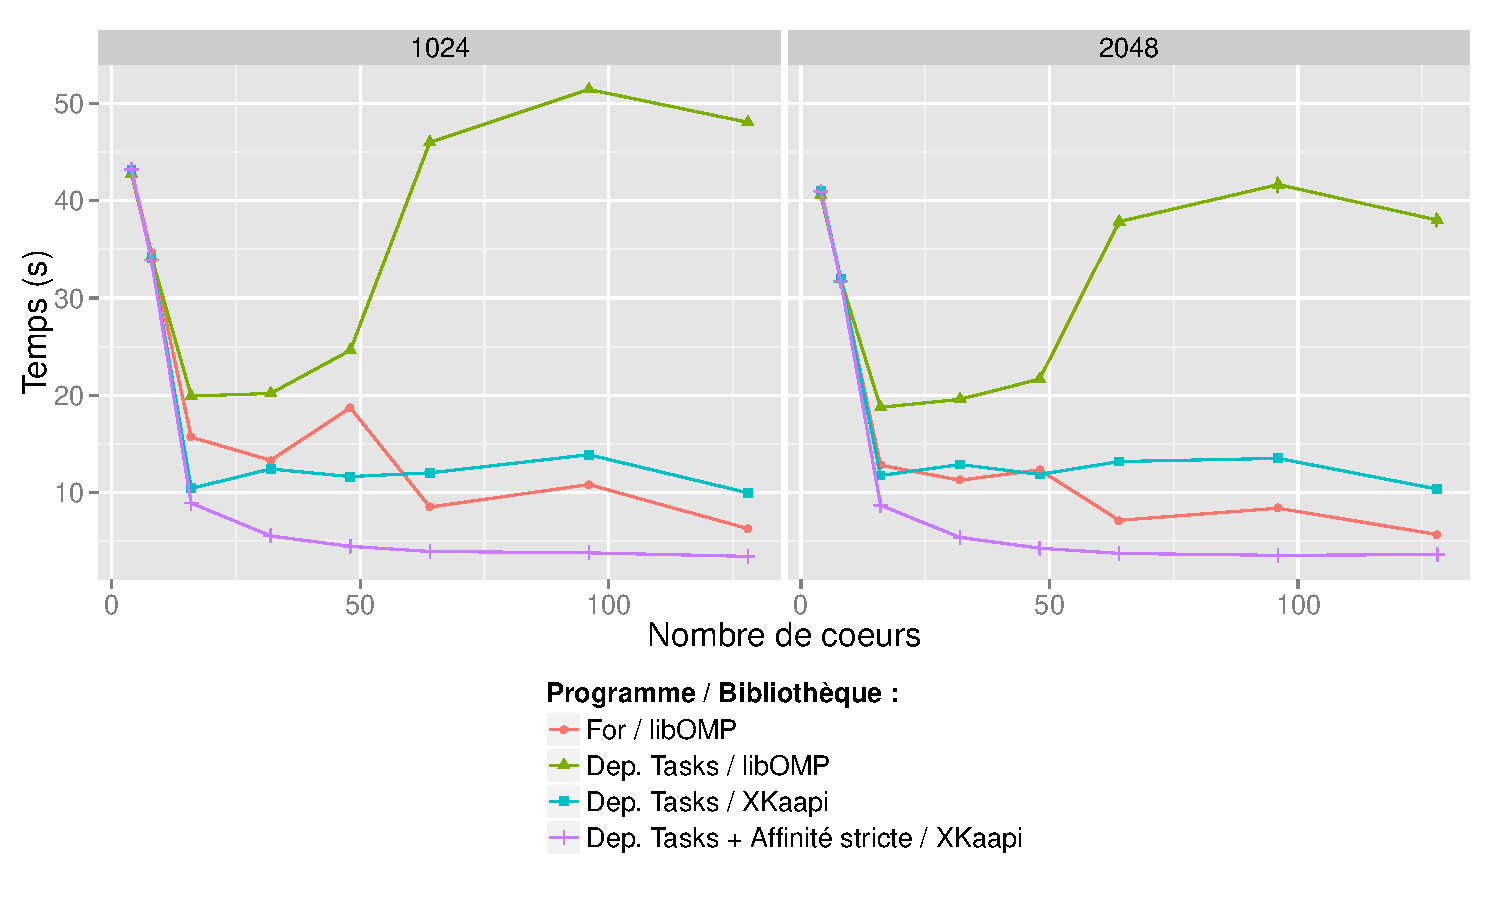
\includegraphics[width=\textwidth]{graph/jacobi_scale_iomp_komp.pdf}
  %\end{center}
  %\uncover<2>{
    %\begin{exampleblock}{Conclusion}
      %c'est possible d'atteindre les performances du \texttt{for} avec des tâches !
    %\end{exampleblock}
  %}
%\end{frame}

%\begin{frame}
  %\frametitle{Evaluating the distributions}
  %\begin{center}
    %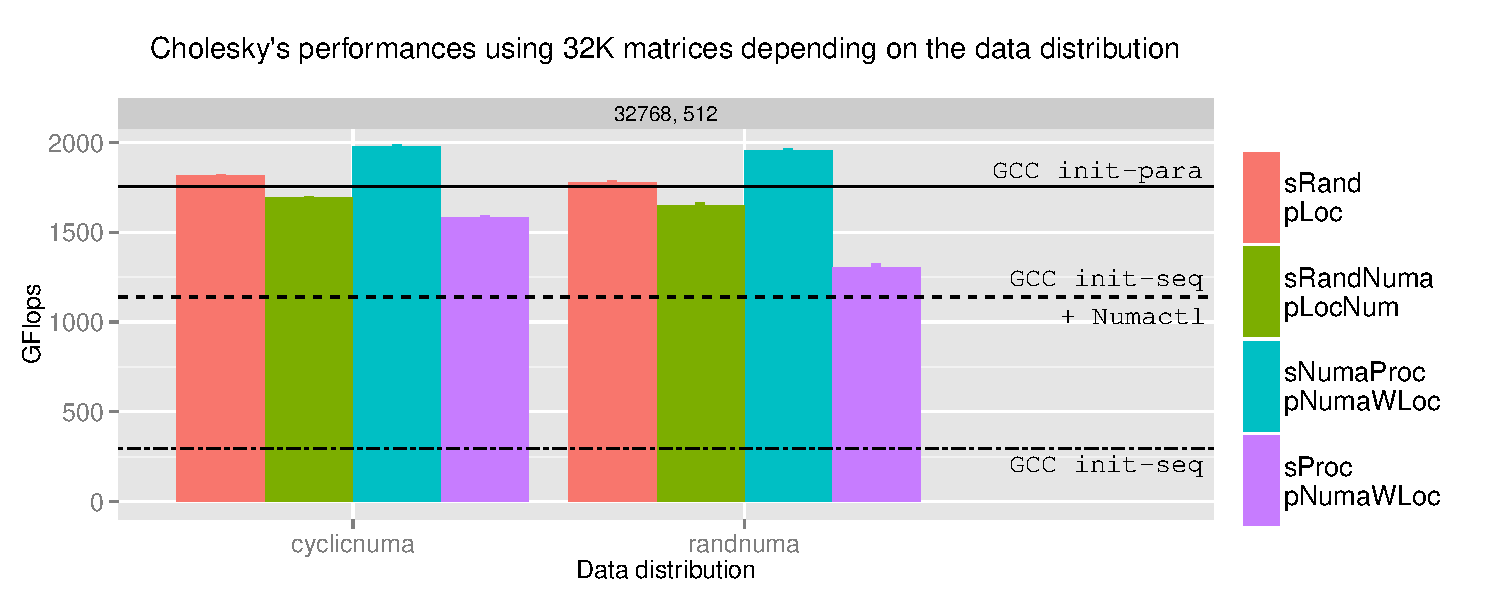
\includegraphics[width=\textwidth]{graph/graph_distrib.pdf}
  %\end{center}
%\end{frame}

%\begin{frame}
  %\frametitle{Évaluation des stratégies (avec cyclicnuma)}
  %\begin{center}
    %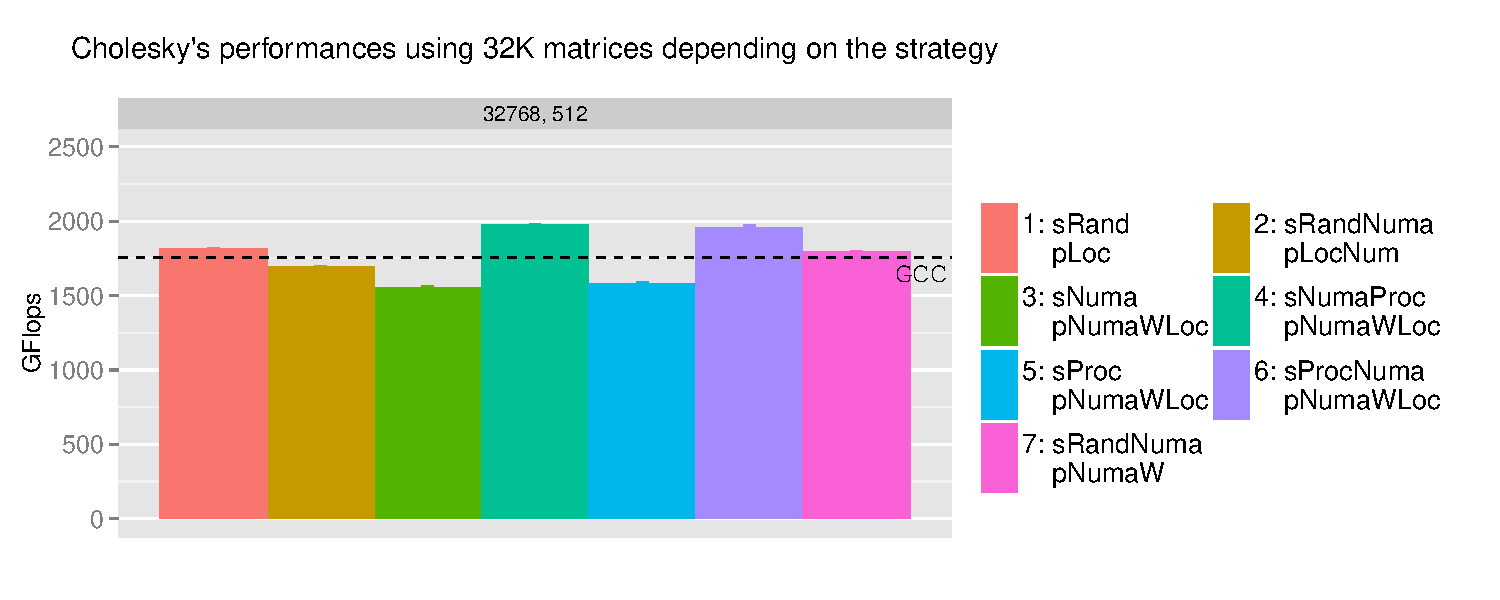
\includegraphics[width=\textwidth]{graph/graph_all_strat.pdf}
  %\end{center}
%\end{frame}

%\begin{frame}
  %\frametitle{Description des trucs évalués}
  %Lister les choses qu'on a pu observer (init, stratégies, etc..)
  %Voir le temps qu'il y a pour parler des différents points
%\end{frame}

%\begin{frame}
  %\frametitle{Cholesky et QR avec une affinité \texttt{data} (idchire)}
  %\footnotesize Matrice : N=32k, BS=512
  %\begin{center}
    %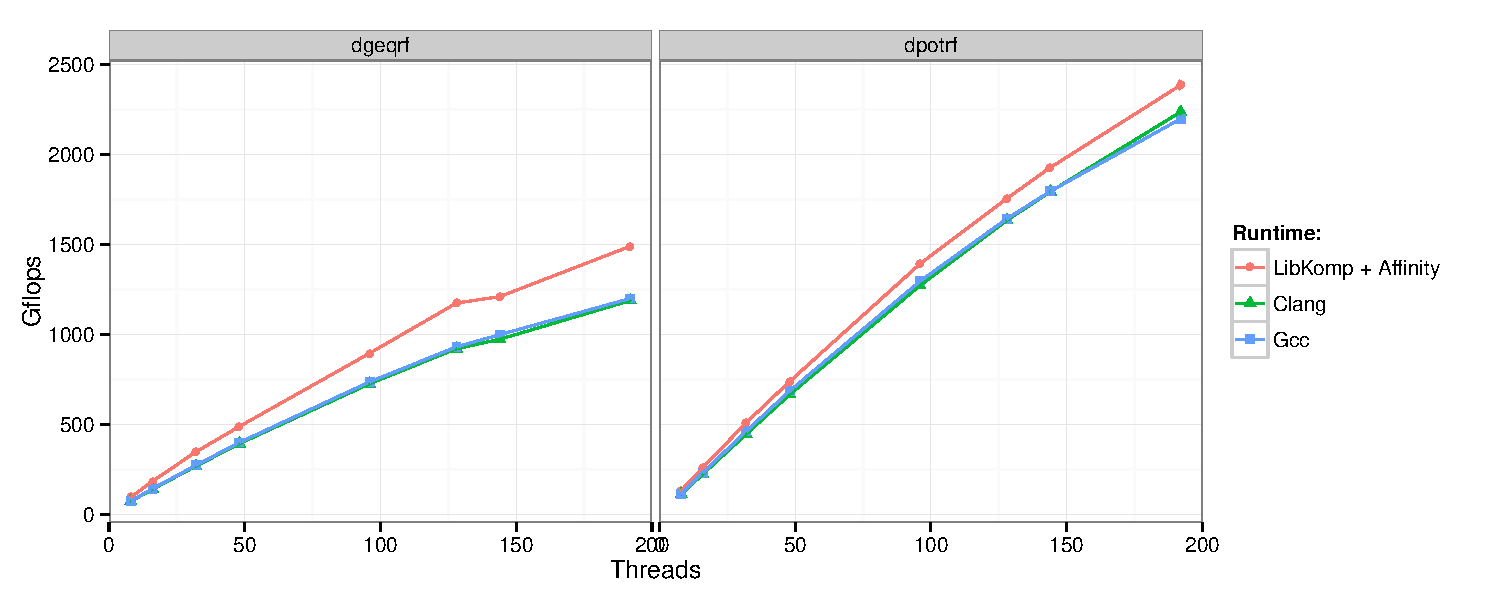
\includegraphics[width=\textwidth]{graph/graph_dpotrf.pdf}
  %\end{center}
%\end{frame}

%\begin{frame}
  %%ça c'est sur idkat : perf équivalente, énergie -- !
  %%737 -> 5602
  %%750 -> 5267
  %%hors RAM -> 340 GFLOPS
  %%6284 - 5866 -> 418
  %% soit environ 80 GFLOPS d'écart -> la DRAM !
  
  %\frametitle{Consommation de la DRAM sur Cholesky (idkat)}
  %\footnotesize Matrice : N=32k, BS=512
  %\begin{center}
    %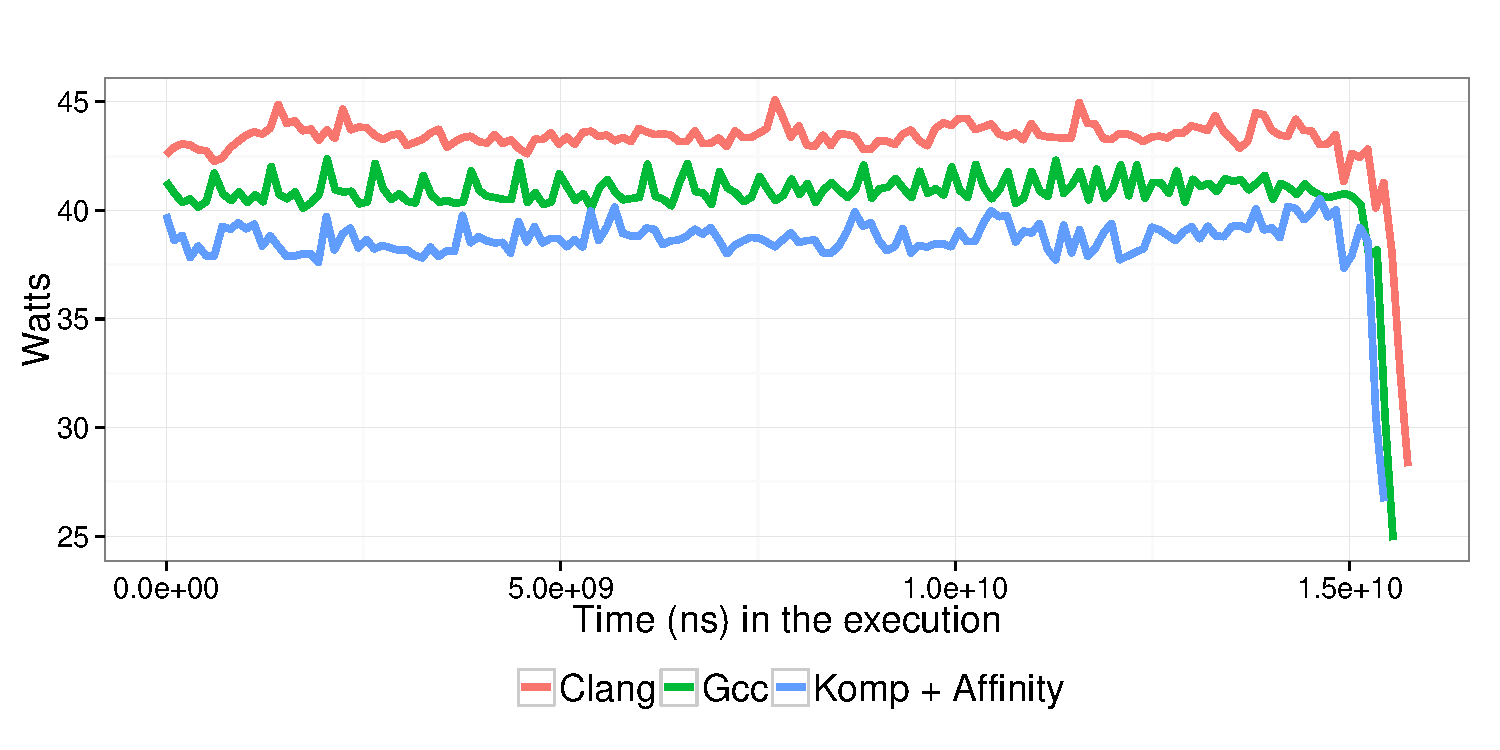
\includegraphics[width=\textwidth]{graph/graph_energy_dram_dpotrf.pdf}
  %\end{center}
%\end{frame}

%\begin{frame}
  
  %\frametitle{Profil énergétique de LU (N=32k, BS=512)}
  %\begin{center}
    %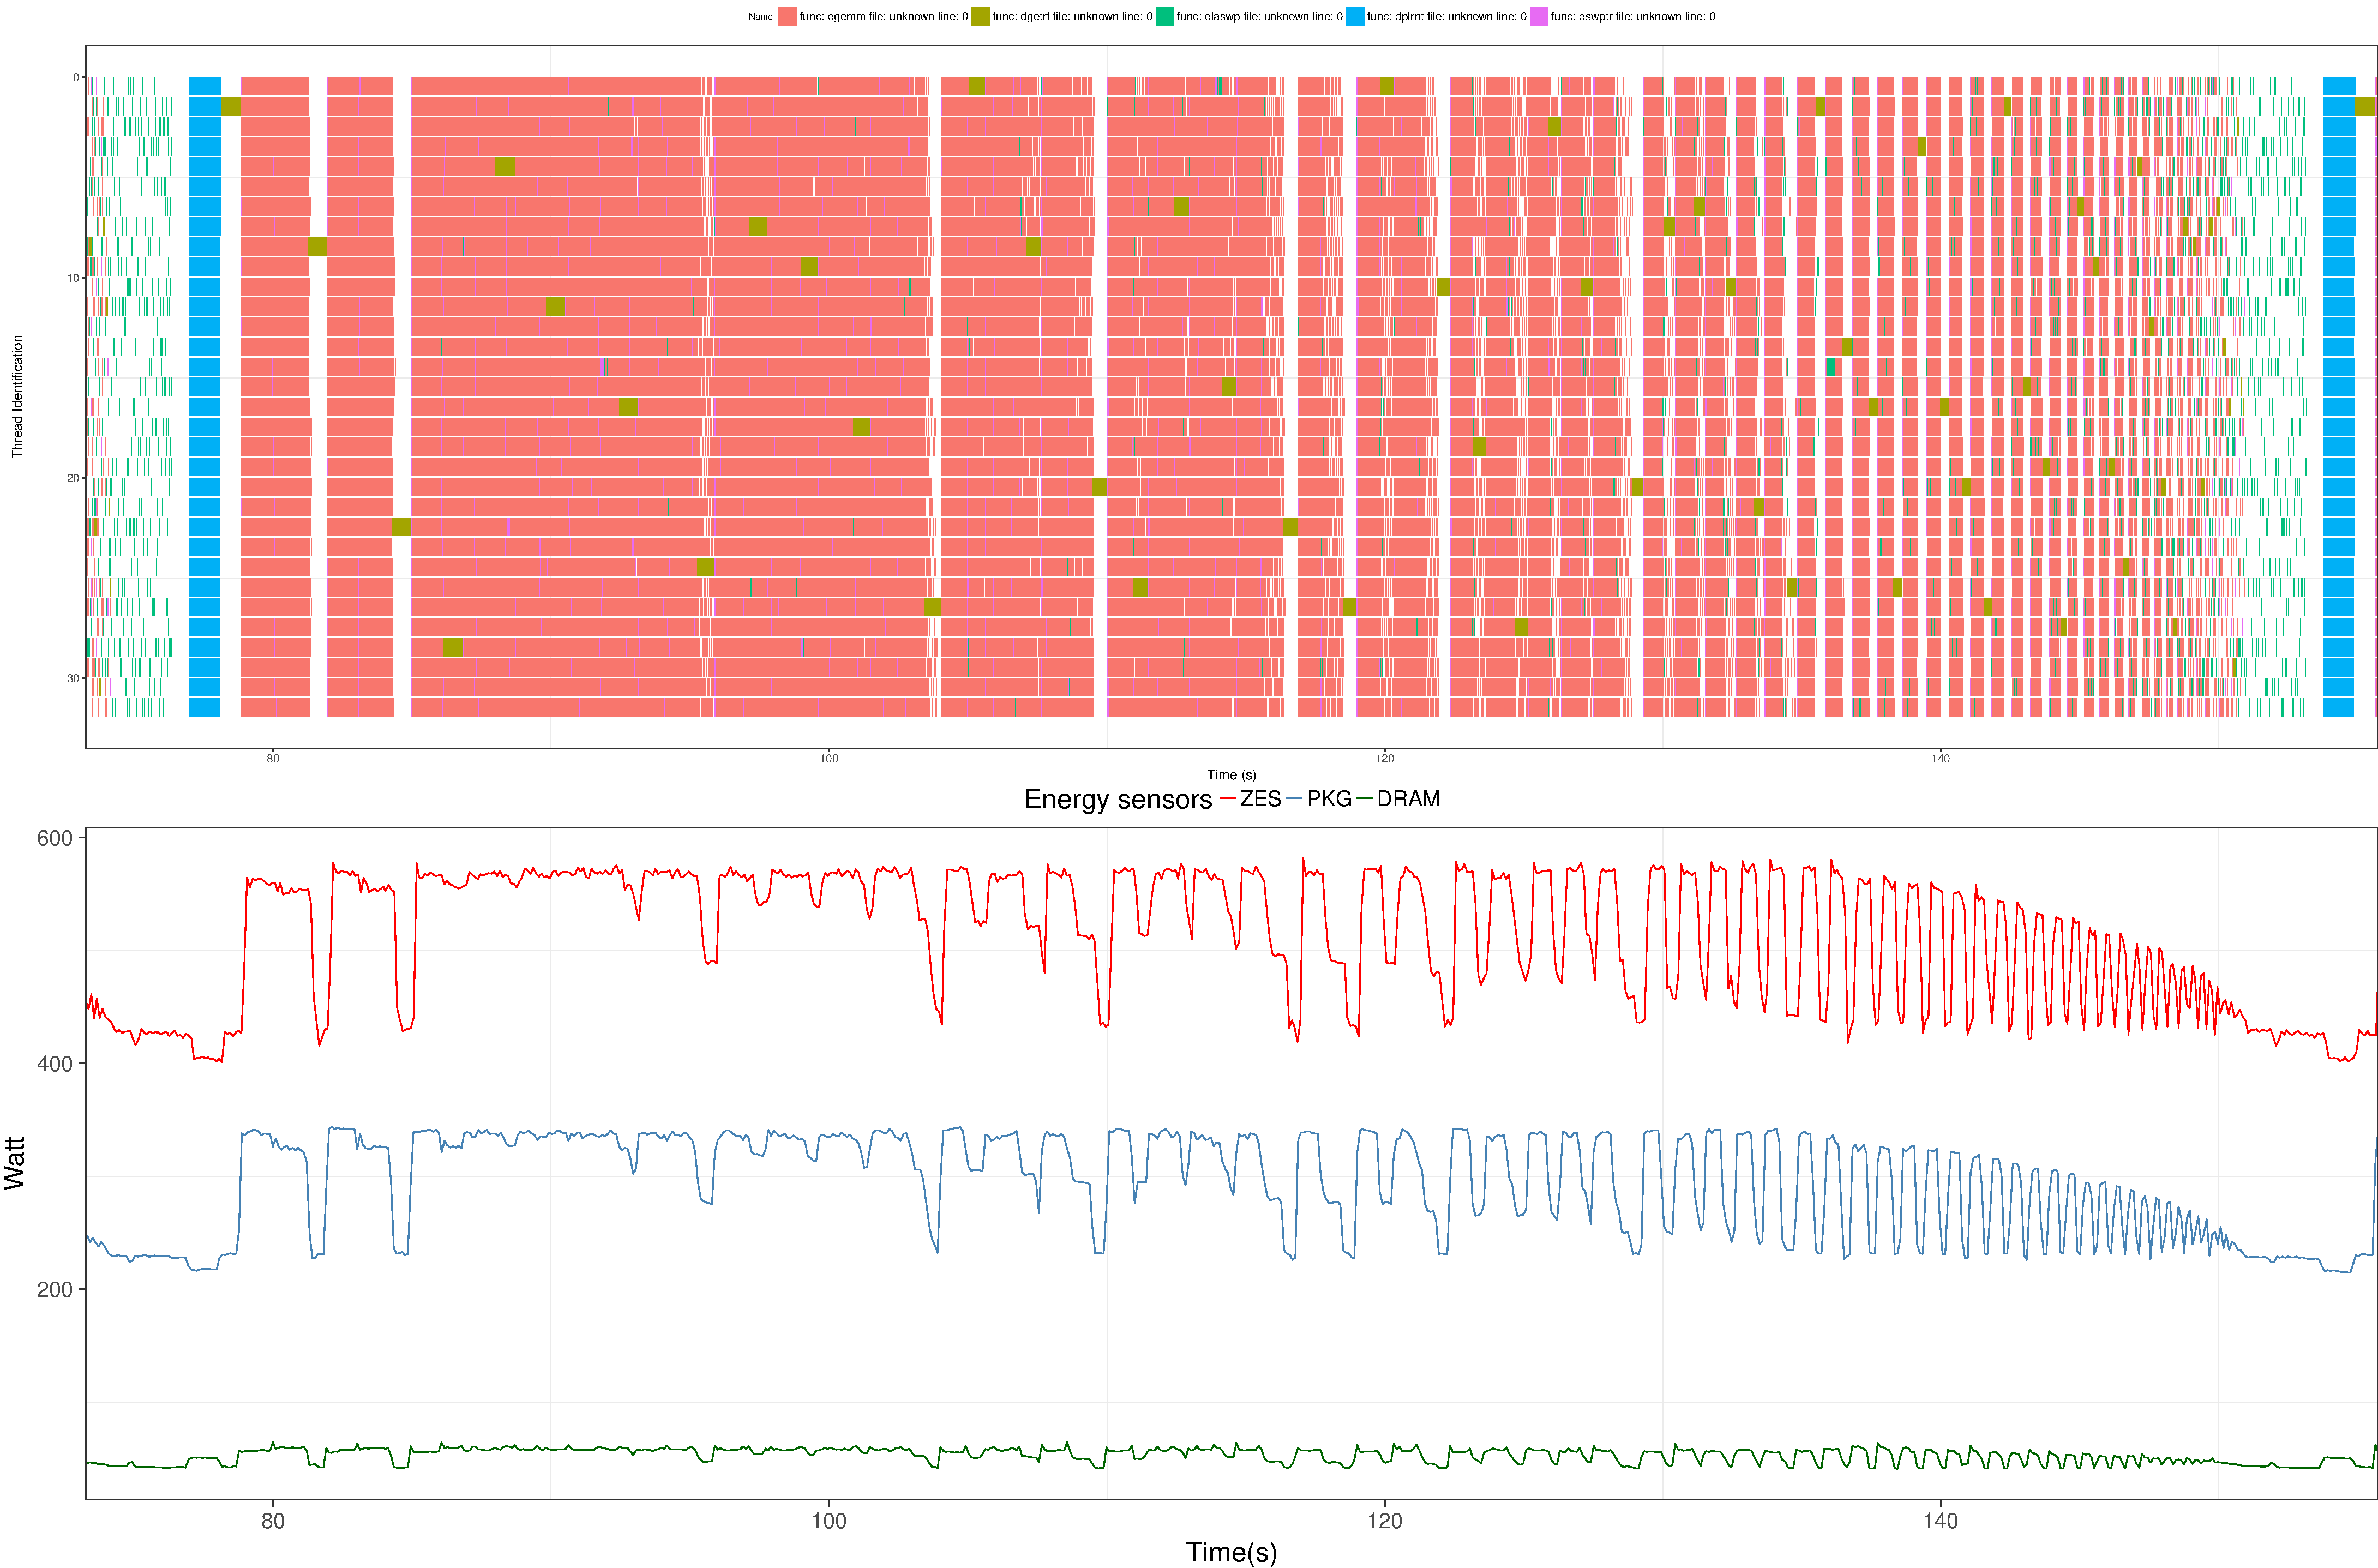
\includegraphics[width=0.8\textwidth]{graph/Rplot.pdf}
  %\end{center}
%\end{frame}


%\begin{frame}[fragile]
  %\frametitle{Conclusion}
  %\begin{block}{Affinité et localité}
    %\begin{itemize}
      %\item Problème de performance identifié et résolu
      %\item Effet "bonus" sur l'énergie
    %\end{itemize}
  %\end{block}

  %\begin{center}
    %Peut on faire mieux ?
  %\end{center}
%\end{frame}

%\section{Simulation}








%\begin{frame}
%\frametitle{Trying the easy way}
%\only<1>{
    %\begin{figure}
        %\includegraphics[width=\textwidth]{graph/graph_defaultmkl.pdf}
    %\end{figure}
    %\vspace{-25pt}
    %\tiny OMP\_NUM\_THREADS=n ./kernel size
%}
%\only<2>{
    %\begin{figure}
        %\includegraphics[width=\textwidth]{graph/graph_defaultmkl_ref.pdf}
    %\end{figure}
    %\vspace{-25pt}
    %\tiny Pic perf in \textcolor{red}{red} !
%}



%\end{frame}
%\begin{frame}
%\frametitle{Common way of dealing with this...}
%\begin{block}{Thread placement}
    %\begin{itemize}
%\item All on same node : reuse cache, nice if compute bound
%\item All distributed accross the machine : average data access faster
%\item Important : no thread migration !
    %\end{itemize}
%\end{block}
%\uncover<2->{
%\begin{block}{Memory distribution}
    %\begin{itemize}
        %\item All memory on the same node : high contention (cf mkl)
        %\item Memory spread accross the node may reduce contention
        %\item Encourage placement of threads near "their" memory
    %\end{itemize}
%\end{block}
%}
%\uncover<3->{
%\begin{block}{Algorithms input}
    %\begin{itemize}
        %\item Choose appropriate size/blocksize for each problem
    %\end{itemize}
%\end{block}
%}
%\end{frame}

%\begin{frame}
%\frametitle{Explicit threads placement and memory distribution}
    %\begin{figure}
        %\includegraphics[width=\textwidth]{graph/graph_16k_mkl.pdf}
    %\end{figure}
    %\vspace{-15pt}
    %\tiny OMP\_NUM\_THREADS=n KMP\_AFFINITY="granularity=fine,explicit,proclist=[...]" numactl -i (...) ./kernel size
%\end{frame}

%\begin{frame}
%\frametitle{Conclusion}
%\begin{alertblock}{Don't}
    %\begin{itemize}
%\item Let the system decide threads placement
    %\end{itemize}
%\end{alertblock}

%\begin{exampleblock}{Do}
    %\begin{itemize}
%\item Pin your threads to avoid migration
%\item Try different threads placement
%\item Control data initialization and distribution
    %\end{itemize}
%\end{exampleblock}

%\end{frame}

%\begin{frame}
%\frametitle{What about task-based OpenMP ?}
    %\begin{figure}
        %\includegraphics[width=\textwidth]{graph/graph_16k_allruntimes.pdf}
    %\end{figure}
    %\vspace{-15pt}
    %\tiny Using OMP\_PLACES to pin threads
%\end{frame}

%\begin{frame}
%\frametitle{Chosing the right blocksize}
    %\begin{figure}
        %\includegraphics[width=\textwidth]{graph/graph_16k_512_allruntimes.pdf}
    %\end{figure}
%\end{frame}

%\begin{frame}
%\frametitle{Conclusion}
%\begin{exampleblock}{Do}
    %\begin{itemize}
        %\item Give the right amount of work to your runtime
    %\end{itemize}
%\end{exampleblock}
%\begin{block}{Note}
    %\begin{itemize}
        %\item Runtimes should be able to better exploit small blocksizes
    %\end{itemize}
%\end{block}

%\end{frame}

%\begin{frame}
%\frametitle{Even more obvious on 32K matrices !}
%\only<1>{
    %\begin{figure}
        %\includegraphics[width=\textwidth]{graph/graph_32k.pdf}
    %\end{figure}
%}
%\only<2>{
    %\begin{figure}
        %\includegraphics[width=\textwidth]{graph/graph_32k_512.pdf}
    %\end{figure}
%}
%\end{frame}

%\begin{frame}
%\frametitle{Conclusion}
%\begin{block}{Performances don't rely only on runtime}
    %\begin{itemize}
%\item Be aware of grain
%\item Tune your inputs
    %\end{itemize}
%\end{block}
%\begin{block}{Performances aren't *that* bad}
    %\begin{itemize}
%\item Decent scaling up to $\approx$100 cores
%\item Still a big gap to experimental pic perf (dgemm)
    %\end{itemize}
%\end{block}

%\end{frame}

%\subsection{Some more tuning !}
%\begin{frame}
%\frametitle{Tuning threads placement}
%\begin{block}{Threads placement}
    %\begin{figure}
        %\includegraphics[width=0.8\textwidth]{graph/thread_placement.pdf}
    %\end{figure}
%\end{block}
%\end{frame}


%\begin{frame}[fragile]
%\frametitle{Tuning data distribution}
%\begin{block}{Data initialization}
    %In kastors : initialized accross all the nodes
%\end{block}

%\begin{block}{Distribution at runtime}
    %Using \verb/numactl --interleave=all/
%\end{block}


%\end{frame}

%\begin{frame}
%\frametitle{The big picture...}
    %\begin{figure}
        %\includegraphics[width=\textwidth]{graph/graph_32k_compare_grid.pdf}
    %\end{figure}
%\end{frame}


%\begin{frame}
%\frametitle{Impact of memory distribution + threads placement}
    %\begin{figure}
        %\includegraphics[width=\textwidth]{graph/graph_32k_compare.pdf}
    %\end{figure}
%\end{frame}

%\begin{frame}
%\frametitle{Conclusion}
%\begin{block}{Memory distribution}
    %Actually worst : data is already distributed during initialization
%\end{block}
%\begin{block}{Threads placement}
    %\begin{itemize}
        %\item Not much difference for low and high number of threads
        %\item Nice gain from spreading the threads otherwise
    %\end{itemize}
%\end{block}
%\end{frame}

%\begin{frame}
    %\frametitle{Pic perf summary}
    %\begin{figure}
        %\includegraphics[width=\textwidth]{graph/graph_32k_picperf.pdf}
    %\end{figure}
%\end{frame}
%\begin{frame}
%\frametitle{Overall conclusion}
%\begin{block}{Tuning matters}
    %\begin{itemize}
        %\item Find the right threads placement
        %\item Adapt memory distribution
        %\item Adapt the grain of your application
    %\end{itemize}
%\end{block}
%\end{frame}


%\section{Solving the scalability issue}

%\begin{frame}
%\frametitle{Still some performances to gain}
%\begin{block}{Next step ?}
    %\begin{itemize}
    %\item Improve the algorithm -> cf litterature
        %\item Tune the program to a specific architecture -> not portable
        %\item Improve the runtime/programming model
    %\end{itemize}
%\end{block}
%\end{frame}

%\begin{frame}
%\frametitle{Still some performances to gain}
%\begin{block}{Improving the programming model}
    %\begin{itemize}
    %\item Better architecture aware directives/clauses
        %\item More tools
    %\end{itemize}
%\end{block}
%\begin{block}{Improving the runtime}
    %\begin{itemize}
        %\item Better mapping of data+threads (needs information)
        %\item NUMA aware algorithm (task queue, barrier, etc)
    %\end{itemize}
%\end{block}
%\begin{block}{Ask for compiler help}
    %\begin{itemize}
        %\item Can help automatically detect dependencies, data placement, etc)
    %\end{itemize}
%\end{block}
%\end{frame}

%\begin{frame}[fragile]
    %\frametitle{Conclusion - Current Kaapi state}
%\begin{onlyenv}<1>%
    %Affinity extension, via OpenMP API
    %\begin{lstlisting}
    %[...]
%omp_set_task_affinity( CYCLIC(m,n,6,4), 1 );
%#pragma omp task depend(out:dA[0:ldam*tempnn])
%CORE_dplgsy( bump, tempmm, tempnn, dA, ldam, A.m, m*A.mb, n*A.nb, seed );
    %[...]
%\end{lstlisting}
%Using Klang-omp :
    %\begin{lstlisting}
    %[...]
%#pragma omp task depend(out:dA[0:ldam*tempnn]) affinity( CYCLIC(m,n,6,4) )
%CORE_dplgsy( bump, tempmm, tempnn, dA, ldam, A.m, m*A.mb, n*A.nb, seed );
    %[...]
%\end{lstlisting}
%\end{onlyenv}
%\only<2>{
    %\begin{figure}
        %\includegraphics[width=\textwidth]{graph/graph_32k_512_kaapi.pdf}
    %\end{figure}
%}
%\footnotesize Reminder : target architecture has 24 (4*6) NUMA nodes.
%\end{frame}

%\begin{frame}
    %\frametitle{Fin}
    %\begin{center}
    %Fin
    %\end{center}
%\end{frame}


%\appendix

%\begin{frame}
%\frametitle{Other ongoing works}
%\begin{block}{Using OMPT}
    %\begin{itemize}
%\item IOMP + HPCToolkit
%\item OMPT can be used to gather information about where a thread fetch its data from.

%\item We want a per-task view
    %\end{itemize}

%\end{block}
%\end{frame}

%\begin{frame}
    %\frametitle{Another threads placement (round robin)}
    %\begin{figure}
        %\includegraphics[width=\textwidth]{graph/graph_32k_compare_spreadnode.pdf}
    %\end{figure}
%\end{frame}


\end{document}
